\documentclass[12pt]{article}
\usepackage[utf8]{inputenc}
\usepackage{graphicx}
\usepackage[a4paper, margin=1in]{geometry}
\usepackage{fancyhdr} % Package to customize the page style
\usepackage{float}
\usepackage[hidelinks]{hyperref}

\usepackage{tocloft}    % For customizing the Table of Contents


\usepackage{amsmath}     % For math expressions
\usepackage{amsthm}      % For theorem environments
\usepackage{hyperref}    % For hyperlinks
\usepackage{caption}     % For customizing captions of tables and figures
\usepackage{longtable}   % For long tables
% Customizing the table of contents (dotted lines and spacing)
\renewcommand{\cftsecleader}{\cftdotfill{\cftdotsep}}  % Add dotted lines to sections





\begin{document}

% First Page (Title Page)
\begin{titlepage}
    \centering
    
\includegraphics[width=5cm]{Picture1.jpg} % Adjust the width if needed to match the size in the image
    
    \vspace{1cm}
    
    \vspace{1.5cm}
    
    \textbf{\Huge Personal Cash Flow Navigator}
    
    \vspace{1cm}
    
    \textbf{\large Bachelor of Science in Computer Science}
    
    \vspace{1cm}
    
    \begin{tabular}{c}
        \textbf{Muhammad Sirat Wali khan} \\
        01-135211-059 \\
        \\
        \textbf{Mahnoor Khan} \\
        01-135211-096 \\
    \end{tabular}
    
    \vspace{2cm}
    
    \textbf{Supervisor: Dr. Kabeer Ahmad Bhatti}
    
    \vfill
    
    \textbf{Department of Computer Science} \\
    Bahria University, Islamabad \\
    October 2024
    
\end{titlepage}

% Second Page (Image with Copyright at Bottom)
\newpage
\pagestyle{empty} % Remove page numbers
\begin{center}

\end{center}

\vfill % Pushes the copyright text to the bottom of the page

\begin{center}
    \footnotesize \copyright Muhammad Sirat Wali Khan and Mahnoor Khan, 2024
\end{center}

% Third Page (Certificate Page)
\newpage
\pagestyle{empty} % Remove page numbers
\begin{center}
    \Large \textbf{Certificate}
\end{center}

\vspace{1cm}

\noindent
We accept the work contained in the report titled “\textbf{Personal Cash Flow Navigator}”, written by Mr. Muhammad Sirat Wali Khan AND Mrs. Mahnoor Khan as a confirmation to the required standard for the partial fulfillment of the degree of \textbf{Bachelor of Science in Computer Science}.

\vspace{2cm}

\noindent
\textbf{Approved by . . . :}

\vspace{1cm}

\noindent
\textbf{Supervisor:} Dr. Kabeer Ahmad Bhatti (Assistant Professor) \\
\noindent\rule{8cm}{0.4pt}

\vspace{1cm}

\noindent
\textbf{Internal Examiner:} Name of the Internal Examiner (Title) \\
\noindent\rule{8cm}{0.4pt}

\vspace{1cm}

\noindent
\textbf{External Examiner:} Name of the External Examiner (Title) \\
\noindent\rule{8cm}{0.4pt}

\vspace{1cm}

\noindent
\textbf{Project Coordinator:} Dr. Kabeer Ahmad Bhatti (Assistant Professor) \\
\noindent\rule{8cm}{0.4pt}

\vspace{1cm}

\noindent
\textbf{Head of the Department:} Dr. Arif ur Rehman (Sr. Associate Professor) \\
\noindent\rule{8cm}{0.4pt}

\vspace{2cm}

\noindent\rule{8cm}{0.4pt}

\vspace{0.5cm}
\noindent
October, 2024

\newpage
\pagestyle{empty} % Remove page numbers

% Position the Abstract title in the middle of the page vertically
\vspace*{8cm} % Adjust this value to control the vertical position

\begin{center}
    \Large \textbf{Abstract}
\end{center}

\vspace{1.5cm} % Adjust this value to control the space between the title and the content

% Abstract content
\noindent
The goal of this project is to create a machine learning-powered intelligent expense tracking app with an admin panel for simple management. Users can log their daily expenses, categorise them, and view their spending patterns through intuitive graphs in this Flutter-created app. By using machine learning, the app gives personalized advice to help users manage their money better and avoid overspending. It looks at how users spend and offers suggestions to cut costs, like reducing non-essential expenses, adjusting their budget, and finding ways to save more. The admin panel makes it easier to manage user accounts. Overall, this project aims to improve financial management for users while making it simple for admins to oversee the system, creating a reliable and easy-to-use financial tool.


% Set Roman page numbering
\pagenumbering{roman}
\pagestyle{plain} % Ensure the page number is displayed at the bottom

% Acknowledgments Page
\newpage
\setcounter{page}{1} % Set the page number to i

% Position the Acknowledgments title in the correct place
\vspace*{3cm} % Adjust this value to control the vertical position of the title

\begin{flushleft}
    \Large \textbf{Acknowledgments}
\end{flushleft}

\vspace{1cm} % Adjust this value to control the space between the title and the content

% Acknowledgments content
\noindent
We are thankful to Almighty Allah for granting us the wisdom, good health, and well-being needed to complete this report. We sincerely thank Dr. Kabeer Ahmad Bhatti for guiding us through various stages of the project and providing all the necessary resources for our research. We are very grateful to him for his expertise, valuable guidance, and encouragement. This project could not have been completed without his supervision and advice. We also appreciate the support and help from all the faculty members of the department. Lastly, we would like to thank our parents for their constant love, care, and support.

\vspace{1.5cm} % Adjust this value to control the space between the content and authors' details

\noindent
\textbf{AUTHORS NAME:} \\
Muhammad Sirat Wali Khan (01-135211-059) \\
Mahnoor Khan (01-135211-096) \\
Islamabad, Pakistan

\vspace{1cm}

\noindent
October 2024

% Quote Page
\newpage
\setcounter{page}{2} % Set the page number to ii

\vspace*{9cm} % Adjust this value to vertically center the quote

% Quote content
\begin{flushright}
    \emph{"“I am no longer
    \\ accepting the things
    I cannot change
\\
    I am changing the things I cannot accept"}
    
    \vspace{1cm}

    \textbf{}
\end{flushright}
% Add four blank pages with Roman numeral page numbers
\newpage

% Add Table of Contents

\tableofcontents


\newpage
% List of Figures
\listoffigures
\newpage

% List of Tables
\listoftables




\newpage
\setcounter{page}{7} % Set the page number to vii
\pagestyle{plain} % Ensure the page number is displayed at the bottom

\vspace*{3cm} % Adjust this value to control the vertical position of the title

\begin{flushleft}
    \Large \textbf{Acronyms and Abbreviations}
\end{flushleft}

\vspace{1cm} % Adjust this value to control the space between the title and the list

\begin{tabbing}
    % Create tabbed list for acronyms and their meanings
    GUI \hspace{2cm} \= Graphical User Interface \\
    API \> Application Programming Interface \\
    HTTP \> Hypertext Transfer Protocol \\
    SQL \> Structured Query Language\\
    UI \> User Interface \\
    AI \> Artificial Intelligence \\
    ML \> Machine Learning\\
    DB \> Database \\
\end{tabbing}

\newpage
 \pagenumbering{arabic}

\vspace*{2cm} % Adjust this value to control the vertical position of the chapter title

% Chapter title
\noindent
\LARGE \textbf{Chapter 1}

\vspace{0.5cm}

% Section title
\noindent
\section{Introduction}


\vspace{1cm} % Adjust this value to control the space between the title and the content

% Introduction content
\noindent
\normalsize In today’s fast-moving world, managing finance successfully is significant, where people struggle to keep track of their daily spending. Conventional methods like using spreadsheets or writing it down manually lead to mistakes and are prone to errors. As the technology emerges, automated and smart tools are in heightened demand to not only make the whole process of expense tracking easy but also to provide feasible suggestions regarding spending patterns. Using this strategy a new expense tracking app is developed and incorporated with the analytics of machine learning. The application enables the user to handle financial matters more smoothly and make well-informed choices on spending patterns, by exploiting advanced technologies\cite{albrecht2014smarter}.
Furthermore, a centralized admin panel is designed to provide an integrated view of the user and simplify the administrative function. The admin panel will allow administrators to handle the accounts of users. This project intends to add more value for users by providing tailored suggestions to make better financial choices \cite{johri2023expense}


\vspace{1cm} % Adjust this value to control the space before the background section

% Subsection title
\noindent
\subsection{Background}

\vspace{0.5cm}

% Background content
\noindent
\normalsize Personal finance management has become highly modern due to the incoming different digital tools and applications that aimed at facilitating people in tracking and managing their expenditure. Traditional means have failed to provide real-time intelligence and personalized useful financial guidance to the users of such facilities. The emergence of smartphones and advancements in machine learning technologies offer new opportunities to optimize the performance of expense-tracking systems.
In this perspective, the proposal leverages these technologies in developing a tool that bridges the gap in existing facilities by providing a single consolidated facility for easy logging of expenses while offering high-level data analytics and machine learning-based recommendations to users. This approach aims not only at making the process of tracking simpler but also at presenting users with useful information and personalized suggestions in the interest of their financial health improvement \cite{anitha2016easy}


\newpage



% Section title: Problem Statement
\noindent
\subsection{Problem Statement}

\vspace{0.5cm}

\normalsize
\noindent This project tackles several crucial issues in personal expense management. The core concept of this project is to improve and make the process of expense tracking easy which is time-consuming and error-prone if done using a spreadsheet or manually \cite{bozkus2009analytical}. The traditional approaches are not able to provide any real-time views into spending behaviors, which makes it hard for people to observe where the money is flowing and how to manage their spending more smartly.\\
Moreover, the existing digital solutions don’t offer strong features for particular financial circumstances. Conventional tools are causing challenges for many users as they do not adjust to their precise financial situation or offer practical suggestions customized to their spending behavior.\\
The ability of the user to enhance financial stability and make thoroughly analyzed financial decisions is restricted due to this constraint \cite{do2023expense}. Additionally, in the current expense tracking system, the centralized management system is lacking from the perspective of an administrator. It could be challenging to manage multiple users in the case of organizations or personal administrators, as it becomes difficult to enforce policies, monitor activities, and extract valuable insights from consolidated data. The absence of a single platform for complete oversight and analysis makes it harder for individuals and organizations.\\
The project aims to comprehensively meet these challenges by developing an advanced expense-tracking application and a centralized admin panel integrated with machine learning analytics. It will offer intuitive ways for users to log, categorize, and analyze expenses efficiently while utilizing machine learning to provide personalized financial insights and recommendations.\\
Simultaneously, the centralized admin panel plans to improve user account management and enhance administrative oversight. This results in a solid approach to effective financial tracking and management \cite{velmurugan2020expense}


\vspace{1cm}

% Objectives section
\noindent
\subsection{Objectives}

\vspace{0.5cm}

\normalsize
    \begin{itemize}
    \item To provide a mobile application based on Flutter that enables the user to enter their daily expenses with ease. It will allow users to categorize, add amount, or scan receipts from photos for record tracking. The aim is to make tracking expenses easier and straightforward for users to ensure accurate financial records\cite{johri2023expense}.
    
    \item The interactive graphs implemented through innovative data visualization tools within the app assist users in analyzing their spending habits. Users can see the visualization of their expenditure patterns over time. Additionally, to provide personalized recommendations based on user data analysis, various machine learning algorithms are incorporated. These suggestions will offer recommendations and insights to help the user achieve their saving goals by customizing suggestions according to each user’s spending habits.
   \newpage  
    \item Create a centralized admin panel to facilitate administrators to view and manage user data in an efficient way, which guarantees smooth control of application users. 
    Implement a feature that allows the administrator to search users via their phone number so that they can access those user details and management controls.
    
    \item The admin has access to Firebase-powered tools through Flutter's integrated features to handle user issues like password resets. Using Firebase, secure login systems are set up to safeguard user data through encryption, decryption, and routine security audits, ensuring user data remains confidential.
\end{itemize}

\vspace{1cm}

% Scope section
\noindent
\subsection{Project Scope}

\vspace{0.5cm}

\normalsize
\noindent The focus of the project is to build two core elements: a mobile application and a centralized admin panel for an expense tracking system. An assortment of features is included in the flutter-based application, which provides for user registration, secure authentication, classification and quick expense entry, the ability to scan receipts and interactive visuals and machine learning-based tailored financial customization are provisioned to help users understand their spending patterns. The admin panel can oversee the user's income to manage records . This project aims to deliver scalable, reliable and administratively controlled solutions to elevate user financial management and ensure that administrators and end users have a seamless and productive experience.

\vspace{1cm}

% Relevance to Course Modules section
\noindent
\subsection{Application Areas}

\vspace{0.5cm}

\normalsize
\noindent The expense tracking app is integrated with a personalized admin and machine learning analytics. It provides useful tools to the users to who want to manage their finances well, to track their expenses, receive personalized suggestions and want to understand about their spending patterns. This application offers many uses for different groups of industries and users.
Additionally, it offers financial literacy education to multiple companies, schools, banks by providing expense tracking methods and budgeting assistance to employees, clients and students. The diverse needs and requirements are addressed through this application as it can adapt to different organizations and users. It serves as an important resource for anyone looking to improve their financial health \cite{sabab2018eexpense}
\vspace{1cm}

% Relevance to Course Modules section
\noindent
\subsection{Organization of Report}

\vspace{0.5cm}

\normalsize
\noindent This report is organized into multiple sections to thoroughly inspect the project’s objective, methodology, outcome, and scope. The project’s background and significance will be highlighted in the introduction section. Next, the problem description determines the challenges, the project aims to address. The aim of the project and key goals are outlined in the objective section. In the scope section, the boundaries of the project and the key focus area are defined. Next, the application area will explore possible uses and identify who will get benefit from the proposed system \cite{sabab2018eexpense}. The methodology section defines which approaches and strategies are used to develop the admin panel and application. At the end, the report will summarize with a discussion on the effects of the project and the expected results, while offering insights into its potential impact and future paths. 
\newpage
 

\vspace*{2cm} % Adjust this value to control the vertical position of the chapter title

% Chapter title
\noindent
\LARGE \textbf{Chapter 2}

\vspace{0.5cm}

% Section title
\noindent
\section{Literature Review}

\vspace{1cm} % Adjust this value to control the space between the title and the content

% Introduction content
\noindent
\normalsize Technology has been integrated in nearly each area. World has come to be an international village and data travels with the speed of light. Technology has made users very smart and demanding. The user today prefers short cuts to save their time. Handling personal finances can be complicated, hence we need simple and effective system that help user to understand their spending patterns. Existing applications have their own features which do not satisfy all the needs that are necessary. Some does not allow you to scan receipt through photos. Some does not have the module for budget suggestions and predictions.\\
The literature review provides a clear perception of the standards being used in the past and the present. The Personal Cash Flow Navigator aims to help people smartly manage their income and expenses by using AI models, Firebase. In this chapter we will explore the shortcomings of previous financial management systems and how the personal cash flow navigator fill these gaps by developing a comprehensive and unified solution for users. 



\vspace{1cm} % Adjust this value to control the space before the background section

% Subsection title
\noindent
\subsection{Existing System}

\vspace{0.5cm}

% Background content
\noindent
\normalsize Conventional approaches to expense tracking often entail the entry of expenses manually into notebooks or spreadsheets is time-consuming and error-prone. The current systems that track expenses differ widely in their features, target audience and usability\cite{manchanda2012expense}. Some individuals prefer basic applications available on mobile phones or web platforms which generally offer features like budget tracking, basic reporting and expense categorization. However, these may fall short of advanced functionalities for thorough monitoring like machine learning-based analytics and a centralized admin dashboard. \\
Additionally, there are extensive management systems for organizations to manage employee spending and keep track of expenses. This system provides features like enforcement of policies, financial analytics and approval process for expenditures and the analysis of finance through compliance requirements and reporting \cite{velmurugan2020expense}. However, to meet the needs of both individual users and businesses, there is still a need for a more enhanced and accessible expense tracking system. These established systems serve their designated purposes to some extent.
\newpage
\vspace{1cm} % Adjust this value to control the space before the background section

% Subsection title
\noindent
\subsection{Comparative Analysis}

\vspace{0.5cm}

% Background content
\noindent
\normalsize Over the years, the financial management has evolved significantly, making it easier for people to handle their finances. Early approaches were manually writing into notebooks or basic spreadsheets. With the advent of digital tools, the financial management has been made easy for people by integrating features like expense categorization, visual graphs and budget suggestions and budget predictions.\cite{cashflowforecasting}
\vspace{1 cm}
\begin{table}[h!]
    \centering
    \resizebox{\textwidth}{!}{%
        \begin{tabular}{|l|c|c|c|c|c|c|}
            \hline
            Features & Khata Tracker & Kharcha & Money Manager & Spending & Budgetfy & Personal Cash Flow Navigator \\
            \hline
            User Authentication & Yes & Yes & Yes & Yes & Yes & Yes \\
            \hline
            Expense Categorization & Yes & Yes & Yes & Yes & Yes & Yes \\
            \hline
            Visual Graphs & Yes & Yes & Yes & Yes & Yes & Yes \\
            \hline
            Set Goals & No & No & No & No & No & Yes \\
            \hline
            Search Expense & No & No & No & No & No & Yes \\
            \hline
            Scan Receipt & No & No & No & No & No & Yes \\
            \hline
            Budget Prediction & No & No & No & No & No & Yes \\
            \hline
            Budget Suggestions & No & No & No & No & No & Yes \\
            \hline
        \end{tabular}%
    }
    % Manually add the second caption below the table
    \begin{center}
        \caption{Comparative Analysis}
    \end{center}
\end{table}

\vspace{1cm} % Adjust this value to control the space before the background section

% Subsection title
\noindent
\subsection{Machine Learning In Financial Management System}

\vspace{0.5cm}

% Background content
\noindent
\normalsize Machine learning has played a crucial role in improving the capabilities of financial management. Machine learning helps users to make informed decisions by analyzing the users past spending patterns. It provides tailored recommendations and predicts future expenses. These features assist users in a smarter way to manage their money effectively.

\vspace{1cm} % Adjust this value to control the space before the background section

% Subsection title
\noindent
\subsection{Scan receipt in financial management system}

\vspace{0.5cm}

% Background content
\noindent
\normalsize Scan receipt is a key feature that helps in automating expense tracking. It uses OCR technology to read from the receipt image and extract the data. The user can simply scan the receipt through photo instead of writing the expense manually.



\vspace{1cm} % Adjust this value to control the space before the background section
% Subsection title
\noindent
\subsection{Search expense in financial management system}

\vspace{0.5cm}

% Background content
\noindent
\normalsize By offering this easy and flexible search feature, the app helps users stay organized, monitor specific expenses, and better understand their spending patterns. It supports better decision-making and allows users to manage their money more effectively by giving them a clear and accurate overview of their financial data, all in just a few taps. This feature allows users to search their expenses easily by category or date, enabling them to access the information they need to manage their money more efficiently.

\vspace{1cm} % Adjust this value to control the space before the background section

% Subsection title
\noindent
\subsection{Gaps in exisitng system}

\vspace{0.5cm}

% Background content
\noindent
\normalsize Despite the availability of contemporary tools, many existing applications still don’t provide a complete solution. For instance, the majority of existing solutions lack features like receipt scanning or budget suggestions that are essential for fully managing money. Additionally, the lack of options like searching for expenses and getting tailored financial advice makes it difficult for users to manage their finances properly. These gaps demonstrate a need for a more comprehensive solution that accommodates various user needs through advanced technologies.




\vspace{1cm} % Adjust this value to control the space before the background section
% Subsection title
\noindent
\subsection{Conclusion}

\vspace{0.5cm}

% Background content
\noindent
\normalsize The current applications provide valuable features but struggle to deliver a customize and scalable user experience. However, the proposed system, integrated with machine learning analytics, bridge these gaps and provide a highly personalized and scalable user experience. Features like tailored financial   suggestions, receipt scanning and budget prediction will create a more efficient and effective solution for user to manage their finances. 
\newpage
 

\vspace*{1.5cm} % Adjust this value to control the vertical position of the chapter title

% Chapter title
\noindent
\LARGE \textbf{Chapter 3}

\vspace{1 cm}

% Section title
\noindent
\section{Requirement Specifications}

\vspace{0.5cm} % Adjust this value to control the space between the title and the content

% Introduction content
\noindent
\normalsize System requirements are configurations that a system needs in order to function properly and effectively. Failure to comply with these requirements may cause installation issues or performance issues. System requirements are documents or sets of documents that outline the features and behavior of a system or software application. 

\vspace{0.5cm} % Adjust this value to control the space before the background section

% Subsection title
\noindent
\subsection{Proposed System}


% Background content
\noindent
\normalsize The intended system looks to provide a robust and intuitive platform with integrated machine learning analytics and a unified admin dashboard to improve the existing system. The mobile application will offer a smooth and effortless experience to user by categorizing expenses, scan their receipt through photos, set their goals, provide visuals of spending through graphs, search their expenses and based on machine learning algorithms they can get budget suggestions and budget predictions to manage their finances effectively\cite{albrecht2014smarter}.
Moreover, the administrator can manage and oversee user details through the centralized admin panel. To access the real time data of users, the admin panel is connected to firebase database system. A complete and scalable solution is provided for managing finances and expense tracking by combining the mobile application and admin panel to cater the needs of both individual user and organizations.\cite{cashflownavigator}
\vspace{1cm} % Adjust space before the image if needed

\begin{figure}[H] % Use [H] to enforce placement here
    \centering
    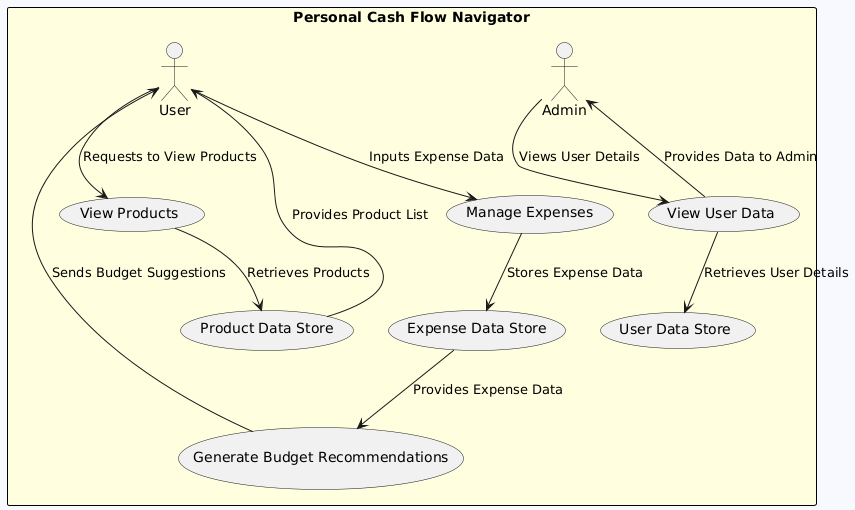
\includegraphics[width=0.8\textwidth]{proposedsystem.png} % Adjust width as needed and replace 'workflow.jpeg' with your image file name
% Manually add the second caption below the table
    \begin{center}
        \caption{Proposed System}
    \end{center}
\end{figure}
\vspace{1cm} % Adjust this value to control the space before the background section

% Subsection title
\noindent
\subsection{Requirement Identifying Techniques}

\vspace{1 cm} % Adjust this value to control the space before the background section
\noindent
\subsubsection{Develop SRS}
\vspace{0.5 cm}

% Background content
\noindent
\normalsize Mention requirements both functional and nonfunctional and software development specifications in the document, also domain requirements. SRS includes the scope, purpose, and introduction of the project.
\vspace{1 cm} % Adjust this value to control the space before the background section

% Subsection title
\noindent
\subsection{Functional Requirements}

\vspace{0.5cm} % Adjust this value to control the space before the background section
\noindent
\normalsize

\textbf{User Authentication}
\begin{itemize}
    \item Users can register and log in securely to use the functionalities of applications.
\end{itemize}

\textbf{Add Expense}
\begin{itemize}
    \item The application allows users to add new expenses to the existing categories or in “other” categories if no category is suitable.
\end{itemize}

\textbf{Expense Visuals}
\begin{itemize}
    \item The spending patterns of users can be seen through visual graphs.
\end{itemize}

\textbf{Search Expense}
\begin{itemize}
    \item The application allows users to search their expenses through date or category.
\end{itemize}

\textbf{Budget Suggestions}
\begin{itemize}
    \item Based on past spending behavior, the user can get budget suggestions for future spending.
\end{itemize}

\textbf{Scan Receipt}
\begin{itemize}
    \item The user can scan receipts through photos to extract the data of expenses.
\end{itemize}

\textbf{Set Goals}
\begin{itemize}
    \item The user can set goals or opt for scrapping.
\end{itemize}

\textbf{Budget Prediction}
\begin{itemize}
    \item Based on the user’s previous spending patterns, the system predicts the next month’s budget.
\end{itemize}

\textbf{View User Details}
\begin{itemize}
    \item The admin can view the details of the user’s on the centralized admin panel.
\end{itemize}
\vspace{1 cm} % Adjust this value to control the space before the background section

% Subsection title
\noindent
\subsection{Non Functional Requirements}

\vspace{0.5cm} % Adjust this value to control the space before the background section
\noindent
\normalsize

\textbf{Performance (Resource Optimization)}
\begin{itemize}
    \item The application has been optimized to make the best use of available system resources.
\end{itemize}

\textbf{Responsiveness}
\begin{itemize}
    \item The system responds quickly to user actions, reducing delays, particularly when working with functions such as budget estimates and image processing.
\end{itemize}

\textbf{Scalability}
\begin{itemize}
    \item The system is designed to handle a growing number of users and greater datasets while maintaining performance.
\end{itemize}

\textbf{Security}
\begin{itemize}
    \item The app must include secure login techniques to ensure that only the right people may access their financial data.
\end{itemize}

\newpage
\vspace{2 cm} % Adjust this value to control the space before the background section

% Subsection title
\noindent
\subsection{Use Case Diagram}

\vspace{1.5cm} % Adjust this value to control the space before the background section
\noindent
\normalsize
\begin{figure}[H]
    \centering
    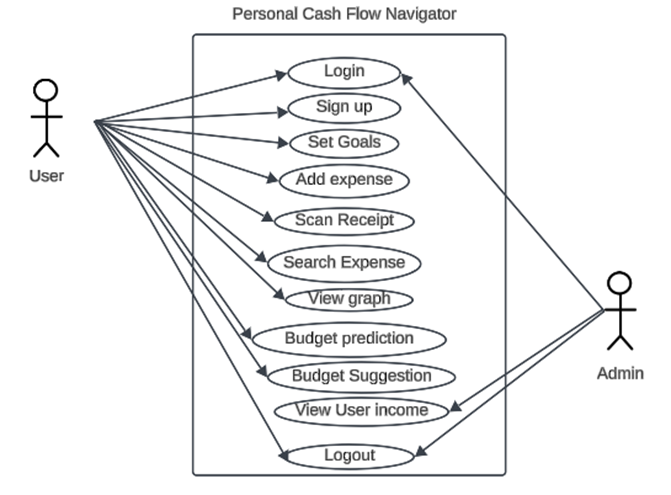
\includegraphics[width=\textwidth]{usecase.png} % Adjust the width to take the full text width, replace 'erd.jpeg' with your image file
 % Manually add the second caption below the table
 \begin{center}
        \caption{Use Case Diagram}
    \end{center}
\end{figure}
\newpage
\vspace{1 cm} % Adjust this value to control the space before the background section

% Subsection title
\noindent
\subsection{Descriptive Use Case}

\vspace{1 cm} % Adjust this value to control the space before the background section
\noindent
\subsubsection{User Signup}
\vspace{0.5 cm}
    % Manually add the second caption below the table
\begin{table}[H] % Use [H] to force the table placement here
    \centering
    \begin{tabular}{|p{4cm}|p{10cm}|}
        \hline
        \textbf{Use Case ID:} & UC-1 \\ \hline
        \textbf{Use Case Name:} & User Signup \\ \hline
        \textbf{Actor(s):} & User \\ \hline
        \textbf{Pre-Conditions:} & 
        1. Application is working. \newline
        2. User has no unique ID. \\ \hline
        \textbf{Priority:} & High \\ \hline
        \textbf{Basic Flow:} & 
        1. User opens the app. \newline
        2. User clicks the button "Sign Up". \newline
        3. System asks for user details. \newline
        4. User enters the details. \newline
        5. System verifies the details. \newline
        6. User sets the password. \newline
        7. System asks for confirmation of the password. \newline
        8. User completes the sign-up process. \\ \hline
        \textbf{Actor Actions:} & 
        \textbf{System Response:} \\ \hline
        User fills out all the required details (name, email, etc.). & 
        System validates and saves the user entry. System displays the message "User added successfully". \\ \hline
        \textbf{Alternative Course of Action (if any):} & \\ \hline
        \textbf{Actor Action:} & \textbf{System Action:} \\ \hline
        1. User is already registered. \newline 
        2. User enters incorrect details. \newline
        3. User sets a weak password. \newline \newline
        4. Confirmation password does not match the original password. & 1. System asks to correct the details.\newline
        2. System requests a stronger password.\newline
        3. System asks for a password reset.\newline\\ \hline 
                
    \end{tabular}
    \caption{Use Case 1: User Signup}
\end{table}


\newpage
\vspace{1 cm} % Adjust this value to control the space before the background section
\noindent
\subsubsection{User Login}
\vspace{0.5 cm}
    % Manually add the second caption below the table
\begin{table}[H] % Use [H] to force the table placement here
    \centering
    \begin{tabular}{|p{4cm}|p{10cm}|}
        \hline
        \textbf{Use Case ID:} & UC-2 \\ \hline
        \textbf{Use Case Name:} & User Login \\ \hline
        \textbf{Actor(s):} & User \\ \hline
        \textbf{Pre-Conditions:} & 
        1. User should have a unique id. \newline
        2. User should have a password. \\ \hline
        \textbf{Priority:} & High \\ \hline
        \textbf{Basic Flow:} & 
        1. User opens the app. \newline
        2. User enters the details. \newline
        3. User clicks the button "Login". \newline
        4. System verifies the details. \newline
        5. User successfully logs into the app. \\ \hline
        \textbf{Actor Actions:} & \textbf{System Response:} \\ \hline
        User fills out all the required login details (unique ID and password).& System validates and allows login if credentials are correct. System displays the message "Login successful". \\ \hline
        \textbf{Alternative Course of Action (if any):} &  \\ \hline
        \textbf{Actor Action:} & \textbf{System Action:} \\ \hline
        1. User enters the wrong unique ID.\newline
2. User re-enters the correct unique ID.\newline
3. User enters the incorrect password. & 1. System prompts to re-enter the correct unique ID.\newline
2. System asks to re-enter the correct password.\newline
3. System displays an error if the server is down and asks the user to try again later.\\ \hline 
                
    \end{tabular}
    \caption{Use Case 2: User Login}
\end{table}



\newpage
\vspace{1 cm} % Adjust this value to control the space before the background section
\noindent
\subsubsection{Admin Login}
\vspace{0.5 cm}
\begin{table}[H] % Use [H] to force the table placement here
    \centering
    \begin{tabular}{|p{4cm}|p{10cm}|}
        \hline
        \textbf{Use Case ID:} & UC-3 \\ \hline
        \textbf{Use Case Name:} & Admin Login \\ \hline
        \textbf{Actor(s):} & Admin \\ \hline
        \textbf{Pre-Conditions:} & 
        1. Admin should have a unique id. \newline
        2. Admin should have a password. \\ \hline
        \textbf{Priority:} & High \\ \hline
        \textbf{Basic Flow:} & 
        1. Admin opens the system panel.\newline
2. Admin enters the details.\newline
3. Admin clicks the button "Login".\newline
4. System verifies the details.\newline
5. Admin successfully logs into the system.\newline \\ \hline
        \textbf{Actor Actions:} & \textbf{System Response:} \\ \hline
        Admin fills out all the required login details (unique ID and password).& System validates and allows login if credentials are correct. System displays the message "Login successful". \\ \hline
        \textbf{Alternative Course of Action (if any):} &  \\ \hline
        \textbf{Actor Action:} & \textbf{System Action:} \\ \hline
       1. Admin enters the wrong unique ID.\newline
2. Admin re-enters the correct unique ID.\newline
3. Admin enters the incorrect password.\newline
4. Server is down, preventing login. & 1. System prompts to re-enter the correct unique ID.\newline
2. System asks to re-enter the correct password.\newline
3. System displays an error if the server is down and asks the Admin to try again later.\\ \hline               
    \end{tabular}
       \caption{Use Case 3: Admin Login}
\end{table}


\newpage
\vspace{1 cm} % Adjust this value to control the space before the background section
\noindent
\subsubsection{Add Expense}
\vspace{0.5 cm}
\begin{table}[H] % Use [H] to force the table placement here
    \centering
    \begin{tabular}{|p{4cm}|p{10cm}|}
        \hline
        \textbf{Use Case ID:} & UC-4 \\ \hline
        \textbf{Use Case Name:} & Add Expense \\ \hline
        \textbf{Actor(s):} & User \\ \hline
        \textbf{Pre-Conditions:} & 
        1. User is logged in.\newline
2. User wants to add a new expense. \\ \hline
        \textbf{Priority:} & High \\ \hline
        \textbf{Basic Flow:} & 
        1. The user is on the dashboard.\newline
2. The user clicks the "Add" button.\newline
3. The expense is validated and saved by the system. \\ \hline
        \textbf{Actor Actions:} & \textbf{System Response:} \\ \hline
        The user enters the expense details and submits the information.& The system validates and saves the expense entry. \\ \hline
        \textbf{Alternative Course of Action (if any):} &  \\ \hline
        \textbf{Actor Action:} & \textbf{System Action:} \\ \hline
      1. System slows down.\newline
2. User clicks the wrong button. & 1. User clicks back and selects the correct button.\newline
- The app may crash.\newline
- System may fail at any time.\newline
1. Restart the app.\\ \hline               
    \end{tabular}
        \caption{Use Case 4: Add Expense}

\end{table}
 
\newpage
\vspace{1 cm} % Adjust this value to control the space before the background section
\noindent
\subsubsection{Scan Invoice through photos}
\vspace{0.5 cm}
    % Manually add the second caption below the table
\begin{table}[H] % Use [H] to force the table placement here
    \centering
    \begin{tabular}{|p{4cm}|p{10cm}|}
        \hline
        \textbf{Use Case ID:} & UC-5 \\ \hline
        \textbf{Use Case Name:} & Scan Invoice through photos \\ \hline
        \textbf{Actor(s):} & User \\ \hline
        \textbf{Pre-Conditions:} & 
        1. User is logged in.\newline
2. User clicks on “Add”.\newline
3. Pre-specified categories are available, or user can select "Other Categories" for unlisted categories.\newline
4. User clicks on "Scan through photos". \\ \hline
        \textbf{Priority:} & High \\ \hline
        \textbf{Basic Flow:} & 
        1. User scans the receipt through photos.\newline
2. The data is extracted by the system.\newline
3. The expense is validated and saved by the system. \\ \hline
        \textbf{Actor Actions:} & \textbf{System Response:} \\ \hline
        User scans the receipt and selects necessary categories.& System extracts, validates, and saves the expense data. \\ \hline
        \textbf{Alternative Course of Action (if any):} &  \\ \hline
        \textbf{Actor Action:} & \textbf{System Action:} \\ \hline
      1. System slows down.\newline
2. User clicks the wrong button. & 1. User clicks back and selects the correct button.\newline
- The app may crash.\newline
- System may fail at any time.\newline
1. Restart the app.\\ \hline               
    \end{tabular}
    \caption{Use Case 5: Scan invoice through photos}
\end{table}


\newpage
\vspace{1 cm} % Adjust this value to control the space before the background section
\noindent
\subsubsection{Search Expenses}
\vspace{0.5 cm}
    % Manually add the second caption below the table
\begin{table}[H] % Use [H] to force the table placement here
    \centering
    \begin{tabular}{|p{4cm}|p{10cm}|}
        \hline
        \textbf{Use Case ID:} & UC-6 \\ \hline
        \textbf{Use Case Name:} & Scan Invoice through photos \\ \hline
        \textbf{Actor(s):} & User \\ \hline
        \textbf{Pre-Conditions:} & 
        1. User is logged in to the app.\newline
2. User is on the dashboard. \\ \hline
        \textbf{Priority:} & High \\ \hline
        \textbf{Basic Flow:} & 1. User clicks on the "Search" button on the dashboard.\newline
2. System displays options to search by date or category.\newline
3. User selects a date range or a category.\newline
4. System filters and displays the relevant expenses based on the search criteria\\ \hline
        \textbf{Actor Actions:} & \textbf{System Response:} \\ \hline
        User selects the search criteria (date range or category) and submits the search.& The system filters and displays the expenses that match the search criteria. \\ \hline
        \textbf{Alternative Course of Action (if any):} &  \\ \hline
        \textbf{Actor Action:} & \textbf{System Action:} \\ \hline
      User enters invalid search criteria. & System should respond quickly.\\ \hline               
    \end{tabular}
        \caption{Use Case 6: Search Expenses}
\end{table}
\newpage
\vspace{1 cm} % Adjust this value to control the space before the background section
\noindent
\subsubsection{Set Goals}
\vspace{0.5 cm}
    % Manually add the second caption below the table
    \begin{center}
        \textbf{Table 3.7: Set Goals}
    \end{center}
\begin{table}[H] % Use [H] to force the table placement here
    \centering
    \begin{tabular}{|p{4cm}|p{10cm}|}
        \hline
        \textbf{Use Case ID:} & UC-7 \\ \hline
        \textbf{Use Case Name:} & Set Goals \\ \hline
        \textbf{Actor(s):} & User \\ \hline
        \textbf{Pre-Conditions:} & 
        1. User is logged in to the app.\newline
2. User is on the dashboard. \\ \hline
        \textbf{Priority:} & High \\ \hline
        \textbf{Basic Flow:} & 1. User is on the Dashboard.\newline
2. User clicks on the "Goals" button.\newline
3. System displays two options: "Set" and "Scraping".\newline
4. User selects one of the options:\newline
- If "Set" is selected: User manually enters financial goals.\newline
- If "Scraping" is selected: System analyzes past spending and savings data to suggest goals automatically.\newline
5. System saves the financial goals and displays them to the user.\\ \hline
        \textbf{Actor Actions:} & \textbf{System Response:} \\ \hline
        User selects the option and sets or receives financial goals.& System saves and displays the financial goals to the user. \\ \hline
        \textbf{Alternative Course of Action (if any):} &  \\ \hline
        \textbf{Actor Action:} & \textbf{System Action:} \\ \hline
      User cancels the goal-setting process. & System should respond quickly.\\ \hline
     \end{tabular} 
     \caption{Use Case 7: Set Goals}
\end{table}



\newpage
\vspace{1 cm} % Adjust this value to control the space before the background section
\noindent
\subsubsection{Budget Suggestions}
\vspace{0.5 cm}
    \begin{table}[H] % Use [H] to force the table placement here
    \centering
    \begin{tabular}{|p{4cm}|p{10cm}|}
        \hline
        \textbf{Use Case ID:} & UC-8 \\ \hline
        \textbf{Use Case Name:} & Budget Suggestions \\ \hline
        \textbf{Actor(s):} & User \\ \hline
        \textbf{Pre-Conditions:} & 
        1. User is logged in to the app.\newline
2. User is on the dashboard.\newline
3. User has historical spending data available in the system. \\ \hline
        \textbf{Priority:} & High \\ \hline
        \textbf{Basic Flow:} & 1. User clicks on the "Budget Suggestions" button.\newline
2. System suggests a budget tailored to the user’s financial behavior.\\ \hline
        \textbf{Actor Actions:} & \textbf{System Response:} \\ \hline
        User requests budget suggestions based on financial history.& System provides personalized budget suggestions based on the user’s financial data. \\ \hline
        \textbf{Alternative Course of Action (if any):} &  \\ \hline
        \textbf{Actor Action:} & \textbf{System Action:} \\ \hline
      1. User cancels the actions.\newline
2. System returns to the previous screen. & System should respond quickly.\\ \hline
     \end{tabular} 
     \caption{Use Case 8: Budget Suggestions}
\end{table}



\newpage
\vspace{1 cm} % Adjust this value to control the space before the background section
\noindent
\subsubsection{View graph of expenses}
\vspace{0.5 cm}
    \begin{table}[H] % Use [H] to force the table placement here
    \centering
    \begin{tabular}{|p{4cm}|p{10cm}|}
        \hline
        \textbf{Use Case ID:} & UC-9 \\ \hline
        \textbf{Use Case Name:} & View graph of expenses \\ \hline
        \textbf{Actor(s):} & User \\ \hline
        \textbf{Pre-Conditions:} & 
        1. User is logged in to the app.\newline
2. The user has added some expenses. \\ \hline
        \textbf{Priority:} & High \\ \hline
        \textbf{Basic Flow:} & 1. User is on the Dashboard.\newline
2. The system displays an interactive graph representing the user’s expenses.\\ \hline
        \textbf{Actor Actions:} & \textbf{System Response:} \\ \hline
        User views the graphical representation of their expenses.& The system generates and displays an interactive graph of the user's expenses. \\ \hline
        \textbf{Alternative Course of Action (if any):} &  \\ \hline
        \textbf{Actor Action:} & \textbf{System Action:} \\ \hline
      1. User cancels the actions.\newline
2. System returns to the previous screen. & System should respond quickly.\\ \hline
     \end{tabular} 
    \caption{Use Case 9: View graph of expenses}
\end{table}

\newpage
\vspace{1 cm} % Adjust this value to control the space before the background section
\noindent
\subsubsection{Budget prediction for next month}
\vspace{0.5 cm}
    \begin{table}[H] % Use [H] to force the table placement here
    \centering
    \begin{tabular}{|p{4cm}|p{10cm}|}
        \hline
        \textbf{Use Case ID:} & UC-10 \\ \hline
        \textbf{Use Case Name:} & Budget prediction for next month \\ \hline
        \textbf{Actor(s):} & User \\ \hline
        \textbf{Pre-Conditions:} & 
        1. User is on the Dashboard.\newline
2. User clicks on the "Budget Prediction" button for the next month. \\ \hline
        \textbf{Priority:} & High \\ \hline
        \textbf{Basic Flow:} & 1. User is on the Dashboard.\newline
2. User clicks on the "Budget Prediction" button for the next month.
3. System provides a predicted budget for the next month.\\ \hline
        \textbf{Actor Actions:} & \textbf{System Response:} \\ \hline
        User requests a predicted budget for the next month. & The system generates and provides a budget prediction for the next month. \\ \hline
        \textbf{Alternative Course of Action (if any):} &  \\ \hline
        \textbf{Actor Action:} & \textbf{System Action:} \\ \hline
      User returns to the previous screen. & System should respond quickly.\\ \hline
     \end{tabular} 
    \caption{Use Case 10: Budget prediction for next month}
\end{table}



\newpage
\vspace{1 cm} % Adjust this value to control the space before the background section
\noindent
\subsubsection{View User Details}
\vspace{0.5 cm}
    \begin{table}[H] % Use [H] to force the table placement here
    \centering
    \begin{tabular}{|p{4cm}|p{10cm}|}
        \hline
        \textbf{Use Case ID:} & UC-11 \\ \hline
        \textbf{Use Case Name:} & View User Detail \\ \hline
        \textbf{Actor(s):} & Admin \\ \hline
        \textbf{Pre-Conditions:} & 
        1. Admin logs into the system.\\ \hline
        \textbf{Priority:} & High \\ \hline
        \textbf{Basic Flow:} & 1. Admin logs into the system.\newline
2. Admin views a list of users and their income data from the admin panel.\\ \hline
        \textbf{Actor Actions:} & \textbf{System Response:} \\ \hline
        Admin accesses the admin panel and views the income data for users. & System retrieves and displays the income data for all users. \\ \hline
        \textbf{Alternative Course of Action (if any):} &  \\ \hline
        \textbf{Actor Action:} & \textbf{System Action:} \\ \hline
      Admin cancels the action. & System should respond quickly.\\ \hline
     \end{tabular}
    \caption{Use Case 11: View User Details}
\end{table}
\newpage
\vspace{1 cm} % Adjust this value to control the space before the background section
\noindent
\subsubsection{Logout}
\vspace{0.5 cm}
    \begin{table}[H] % Use [H] to force the table placement here
    \centering
    \begin{tabular}{|p{4cm}|p{10cm}|}
        \hline
        \textbf{Use Case ID:} & UC-12 \\ \hline
        \textbf{Use Case Name:} & Logout \\ \hline
        \textbf{Actor(s):} & User \\ \hline
        \textbf{Pre-Conditions:} & 
        User is logged in to the app.\\ \hline
        \textbf{Priority:} & High \\ \hline
        \textbf{Basic Flow:} & . User clicks on the "Log out" button.\\ \hline
        \textbf{Actor Actions:} & \textbf{System Response:} \\ \hline
        User initiates the logout action. & System logs the user out of the application.\\ \hline
        \textbf{Alternative Course of Action (if any):} &  \\ \hline
        \textbf{Actor Action:} & \textbf{System Action:} \\ \hline
      1a. User clicks the wrong button.\newline
1b. User clicks the correct button. & 1. The app may crash.\newline
2. The system may fail at any time.\newline
3. Restart the app.\\ \hline
     \end{tabular}
     \caption{Use Case 12: Logout}
\end{table}

\newpage

\vspace*{1.5cm} % Adjust this value to control the vertical position of the chapter title

% Chapter title
\noindent
\LARGE \textbf{Chapter 4}

\vspace{1 cm}

% Section title
\noindent
\section{Design and Architecture}

\vspace{0.5cm} % Adjust this value to control the space between the title and the content

% Introduction content
\noindent
\normalsize In today's ever changing economic landscape, efficient financial management is imperative. Ineffective financial planning can lead to unexpected costs and poor budgeting which can put businesses and individuals under financial strain and challenges in achieving financial goals. In order to address these issues, the Personal Cash Flow Navigator seeks to assist individuals by
 providing a seamless and convenient platform to manage the finances of users.


Personal Cash Flow Navigator is designed with a modular and scalable architecture by leveraging machine learning analytics and a comprehensive dashboard to accommodate both user and organizations. The application allows user to scan their receipt, categorize their expenses, and receive budget suggestion based on their spending patterns.

\vspace{1cm} % Adjust this value to control the space before the next section

% Subsection title
\noindent
\subsection{External Interface Requirements}

\vspace{0.5 cm} % Adjust this value to control the space before the content
\noindent
\normalsize User can interact with the app by the touch screen. The output will be displayed in a few seconds. Users can click on the to add expenses in the categories, set financial goals,search expenses or scan receipts, and by clicking on budget suggestion option, they can see the budget recommendations.The admin can view user income details through the admin centralized panel.\cite{gupta2020expense}

\vspace{1 cm} % Space before the subsection title
% Sub-subsection title

\noindent
\subsubsection{Software Interfaces}

\vspace{0.5 cm} % Adjust this value to control the space before the content
\noindent
The app will enable user to  enter expenses, establish budget goals and monitor their cash flow using different interfaces.

\vspace{0.5 cm} % Adjust this value to control the space before the list
\noindent
\begin{itemize}
    \item Scan receipt through photos
    \item Search Expense
    \item Financial Insights
    \item Budget Suggestion
    \item Budget Prediction
\end{itemize}
\vspace{0.5 cm} % Space before the next subsection title
% Sub-subsection title
\noindent
\subsubsection{Communication Interfaces}

\vspace{0.5 cm} % Adjust this value to control the space before the list
\noindent
\begin{itemize}
    \item Internet
    \item Login using email
\end{itemize}

\vspace{1cm} % Adjust this value to control the space before the next section

% Subsection title
\noindent
\subsection{Context Diagram}

\vspace{0.5 cm} % Adjust this value to control the space before the content
\noindent
\normalsize The context diagram shows the overview of the proposed system and how it interacts with the external entities. It includes users and admins who utilize the system to add expenses, get personalized suggestions, search expenses, and manage their accounts. It shows how the information flows between the system and the user interacting. It’s a simple way to
understand who and what interacts with the system. 
\vspace{1cm} % Adjust space before the image if needed
   
\begin{figure}[H] % Use [H] to enforce placement here
    \centering
    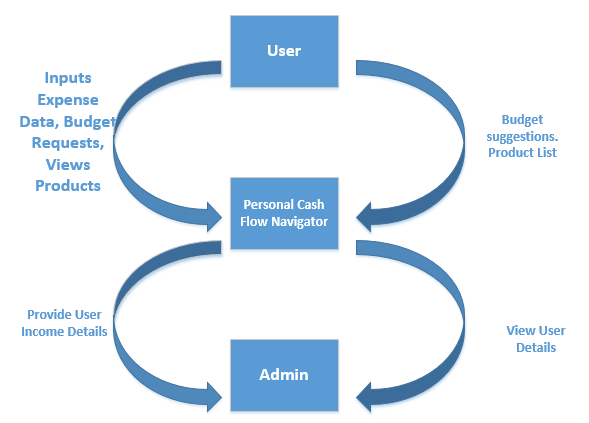
\includegraphics[width=0.8\textwidth]{context.png} % Adjust width as needed and replace 'workflow.jpeg' with your image file name
% Manually add the second caption below the table
 \begin{center}
        \caption{Context Diagram}
    \end{center}
\end{figure}
 

\newpage
\newpage
\vspace{1 cm} % Space before the subsection title
% Sub-subsection title
\noindent
\subsection{Design Constraints}
\vspace{0.5 cm} % Adjust this value to control the space before the list
\noindent

 \normalsize
 There are some design constraints in our project:
 \begin{itemize}
    \item Our Application's user interface must be operational.
    \item Application to be user-friendly.
    \item Response time to be minimum.
    \item Application should be responsive.
\end{itemize}
\vspace{1 cm} % Space before the subsection title
% Sub-subsection title
\noindent
\subsection{Design Methodology}

\vspace{0.5 cm} % Adjust this value to control the space before the list
\noindent
 \normalsize
In design methodology, we define the procedures and techniques which will help us in designing our application. As we have to develop a mobile application, this is why we needed flutter knowledge. The design process always requires iterations and improvements on each level in order to minimize errors in the final product. We brainstormed and encouraged new ideas and collaborative thinking to work through each idea and arrive at the best and optimal solution.\cite{khandelwal2022developing}

\vspace{1 cm} % Space before the subsection title
% Sub-subsection title
\noindent
\subsection{High Level Design}

\vspace{0.5 cm} % Adjust this value to control the space before the list
\noindent
 \normalsize
High level design provides us a detailed overview of how different functionalities and features coordinate and interact with each other. This section highlights the basic workflow along with alternative paths just in case a failure occurs. 
\newpage
\vspace{1 cm} % Space before the subsection title
% Sub-subsection title
\noindent
\subsection{Design Models}

\vspace{0.5 cm} % Adjust this value to control the space before the list
\noindent
 \subsubsection{Architecture Design}

\begin{figure}[H]
    \centering
    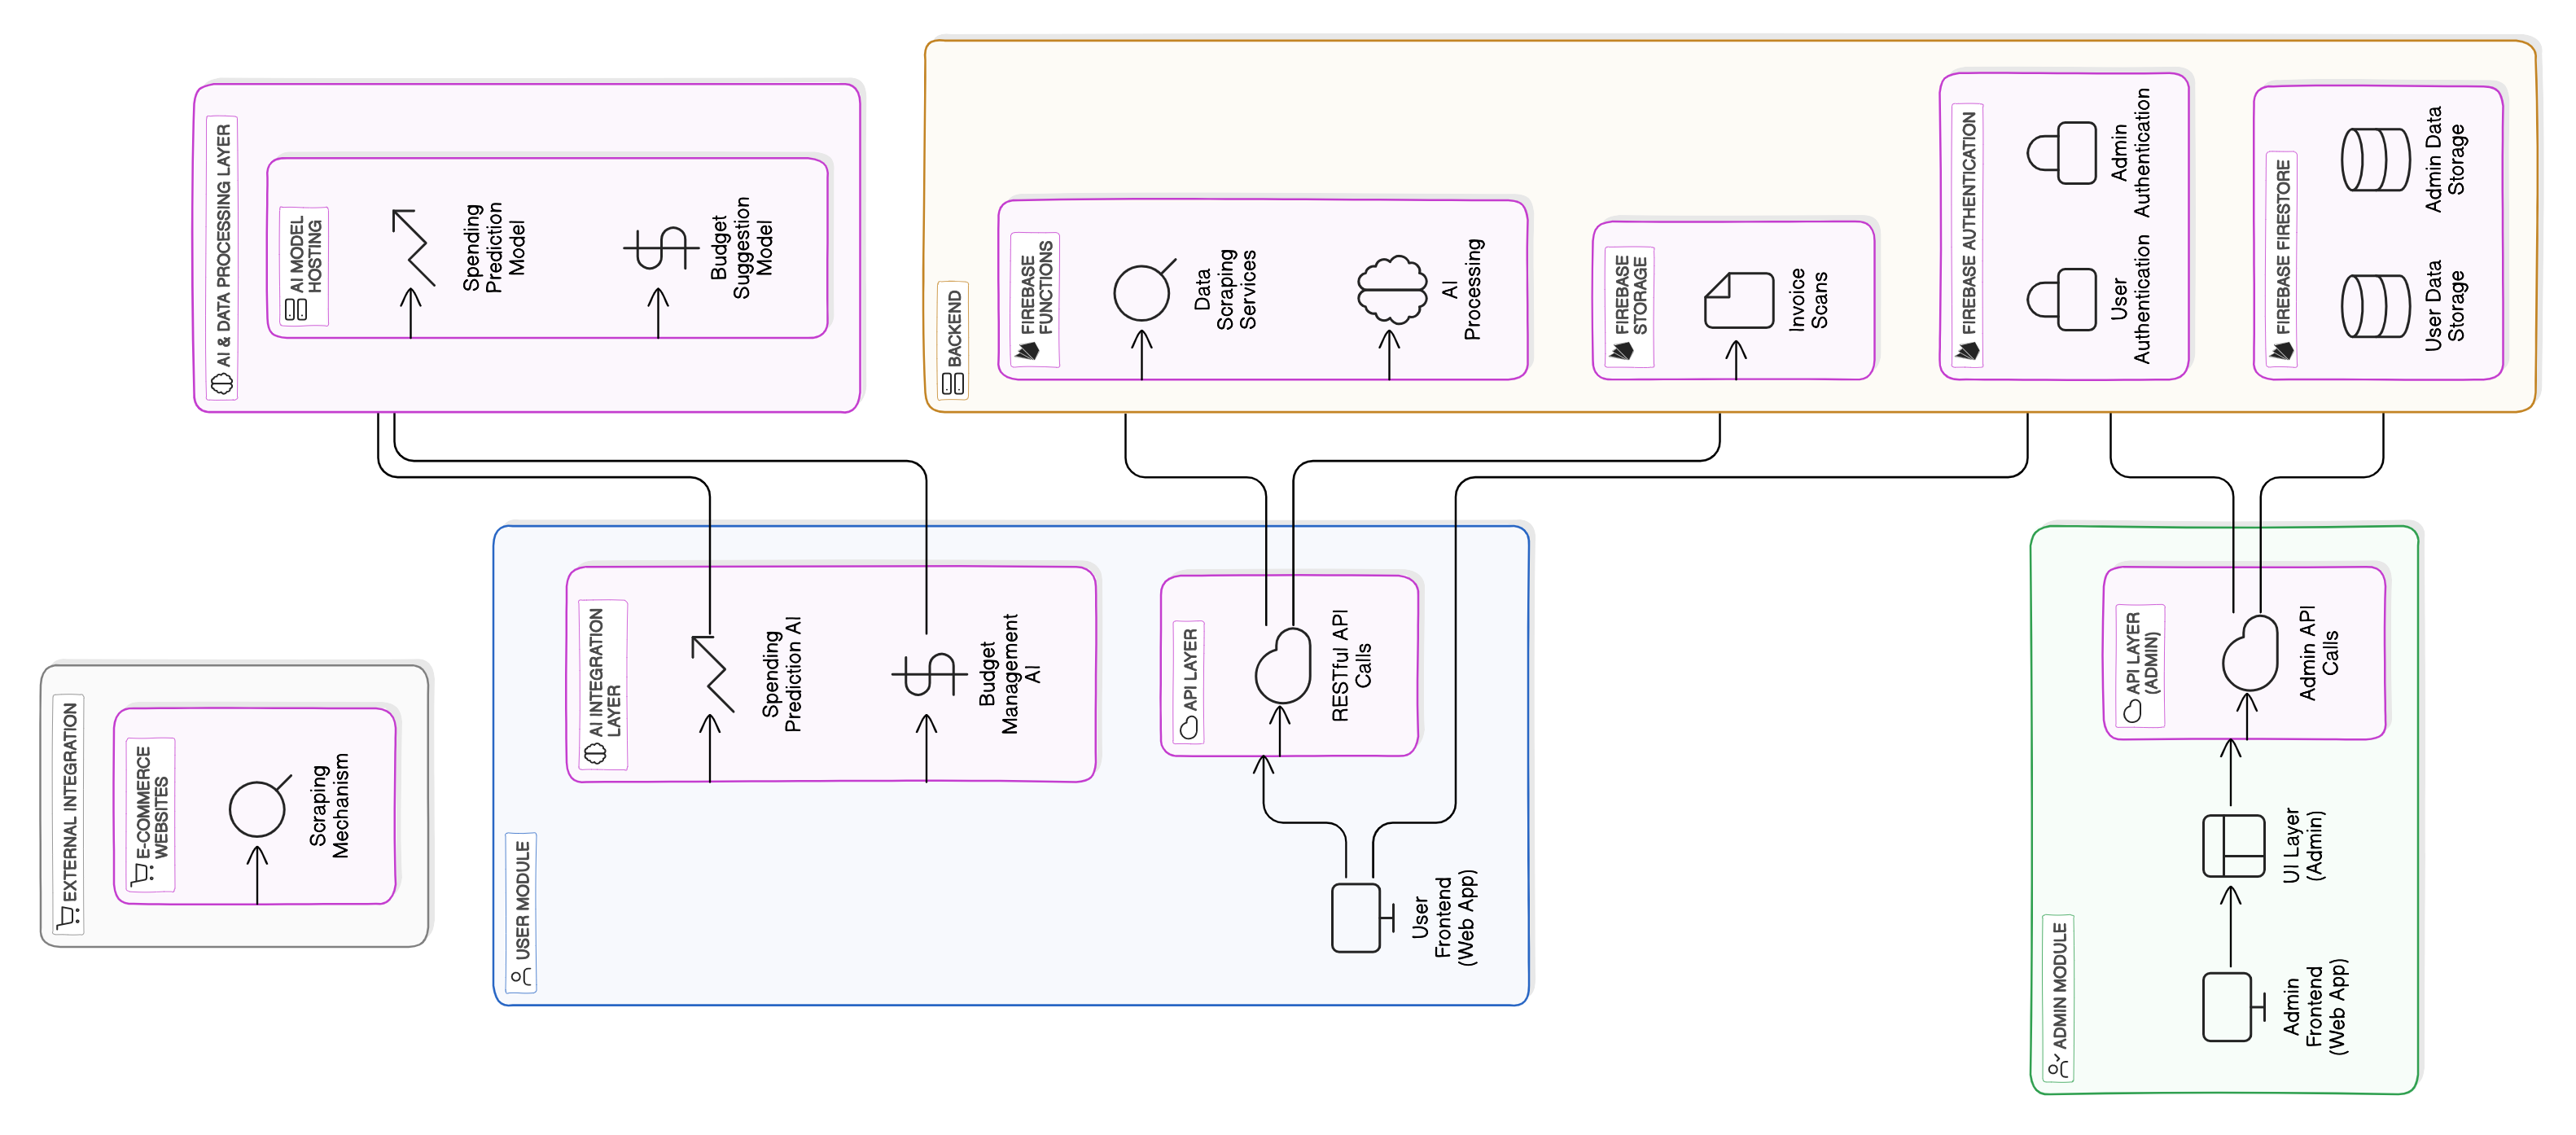
\includegraphics[width=1.0\textwidth]{architectural.png}
\begin{center}
        \caption{Architecture Design}
    \end{center}
\end{figure}
\newpage
\vspace{1cm} % Adjust this value to control the space before the next section

% Subsection title
\noindent
\subsection{Data Flow Diagram}

\vspace{0.5 cm} % Adjust this value to control the space before the content
\noindent
\normalsize It is a tool that provides a clear overview of how the data flows within the personal cash flow navigator. It shows how the external entities like the user, administrator and firebase interact with the system. The main process called the Personal Cash Flow Navigator, connects with multiple external entities to interact with the system.User, being one of the primary external entities can add their expenses to the application, which helps them to keep track of and manage their spending. Additionally, another important external entity is the admin, which is capable of accessing  user information from the system and   handling users . The system also interacts with the Firebase database system to ensure that the user's data is easily accessible and securely stored.
\vspace{1cm} % Adjust space before the image if needed

  

\newpage
\vspace{1cm} % Adjust this value to control the space before the next section

% Subsection title
\noindent
\subsection{Activity Diagram}

\vspace{0.5 cm} % Adjust this value to control the space before the content
\noindent
\normalsize In Personal Cash Flow Navigator activity diagram, first, the system enters a login screen. From there, it goes to a dashboard
screen where the user can choose different options. These options include add spending,scan receipt, visual graphs, budget suggestion, budget prediction or search expense. After the user selects one of these options, it goes through a series of step to finish the task,making sure the selected task is fully carried out.
\vspace{1cm} % Adjust space before the image if needed
\begin{figure}[H] % Use [H] to enforce placement here
    \centering
    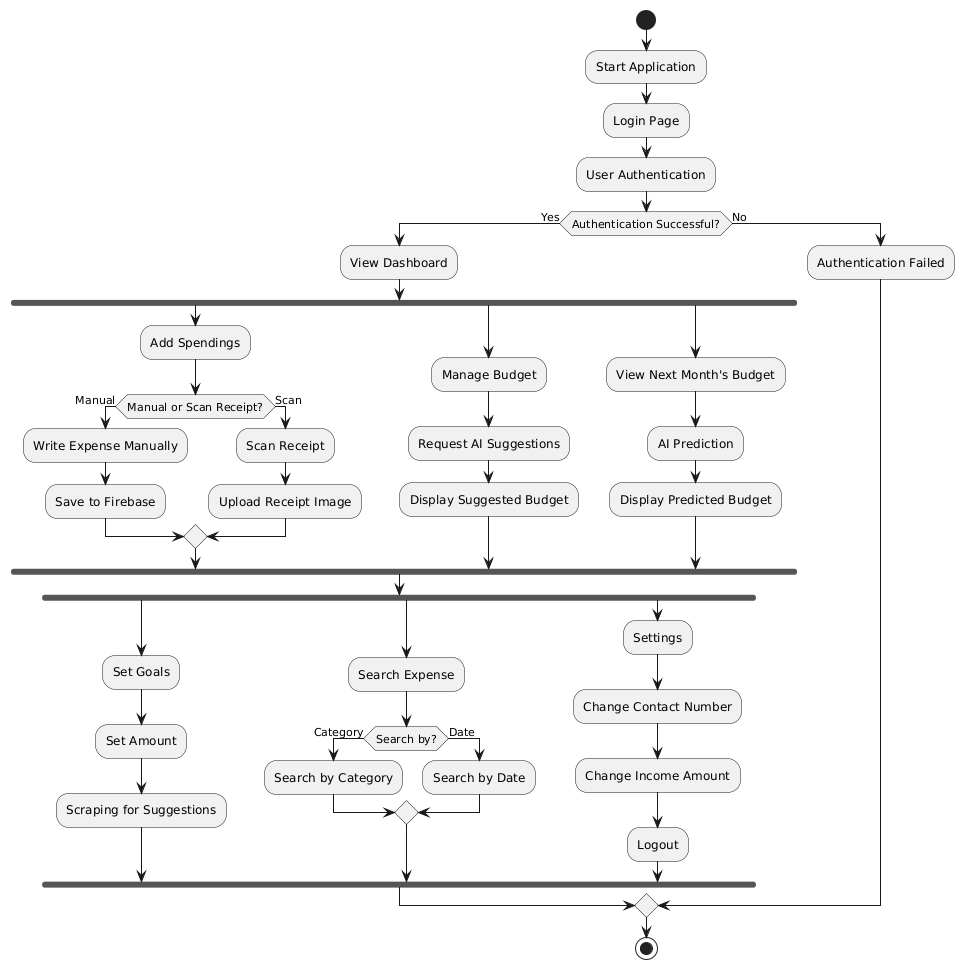
\includegraphics[width=1.0\textwidth]{activitydiagram.png} % Adjust width as needed and replace 'workflow.jpeg' with your image file name
% Manually add the second caption below the table
    \begin{center}
        \caption{Activity Diagram}
    \end{center}
\end{figure}

\newpage
\vspace{1 cm} % Adjust this value to control the space before the background section

% Subsection title
\noindent
\subsection{ERD Diagram}

\vspace{0.5cm} % Adjust this value to control the space before the background section
\noindent
\normalsize

\begin{figure}[H]
    \centering
    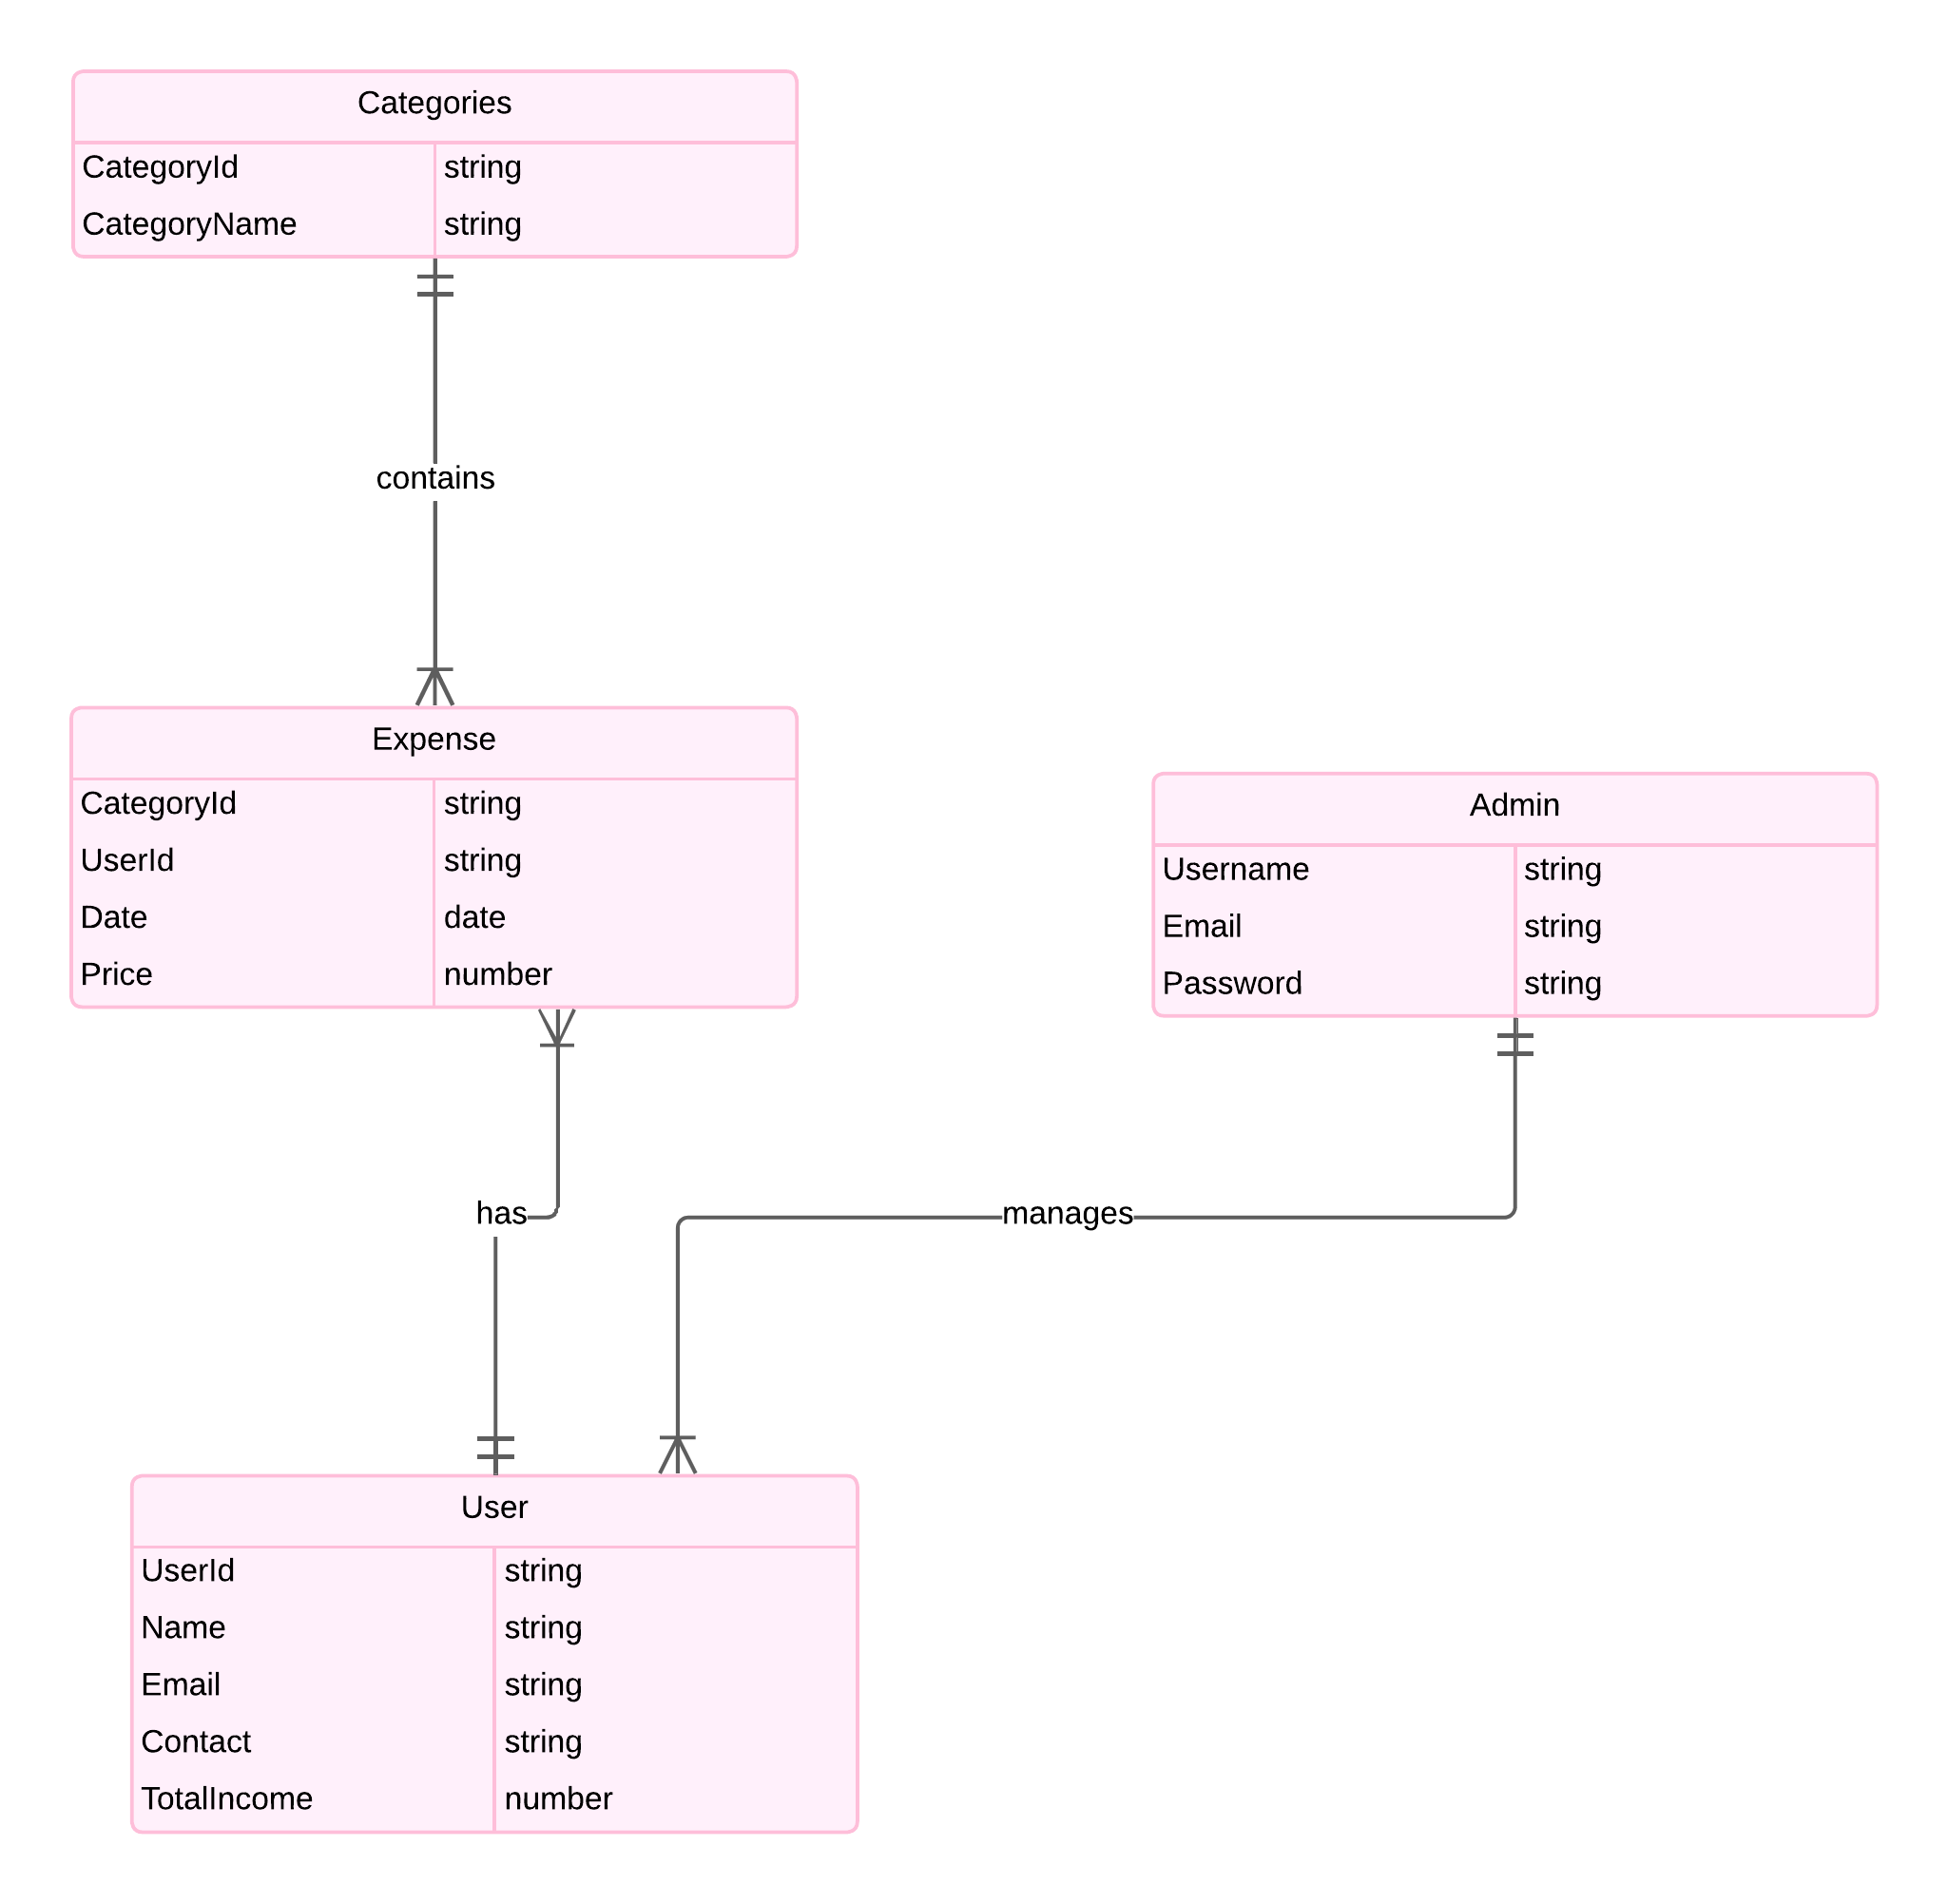
\includegraphics[width=\textwidth]{ERD.png} % Adjust the width to take the full text width, replace 'erd.jpeg' with your image file
 % Manually add the second caption below the table

\begin{center}
    \caption{ERD Diagram}
\end{center}
\end{figure}
\newpage

\vspace{1 cm} % Adjust this value to control the space before the background section

% Subsection title
\noindent
\subsection{Sequence Diagram}

\vspace{0.5cm} % Adjust this value to control the space before the background section
\noindent
\subsubsection{User Sequence Diagram}

\begin{figure}[H]
    \centering
    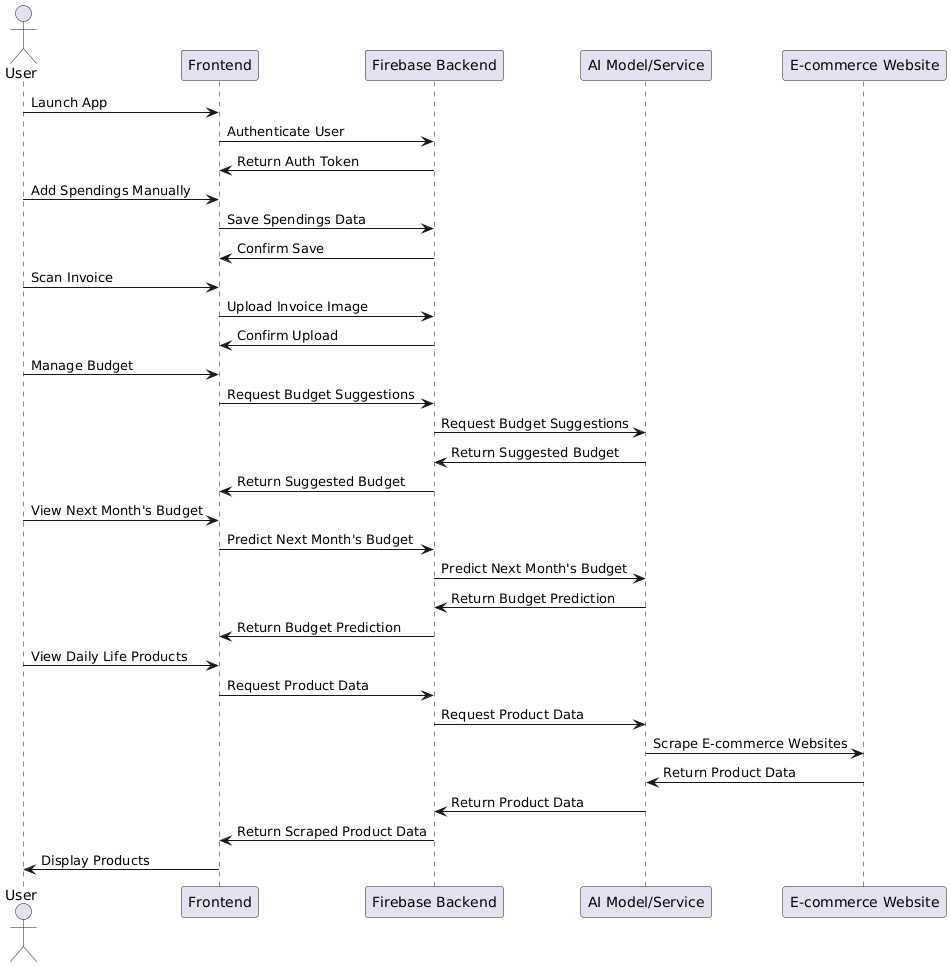
\includegraphics[width=\textwidth]{userseq.png} % Adjust the width to take the full text width, replace 'erd.jpeg' with your image file
 % Manually add the second caption below the table

\begin{center}
    \caption{User Sequence Diagram}
\end{center}
\end{figure}
\newpage

\vspace{1 cm} % Adjust this value to control the space before the background section

% Subsection title
\noindent
\subsubsection{User Login}

\vspace{0.5cm} % Adjust this value to control the space before the background section
\noindent
\normalsize This diagram shows how the user can log in to the application. The user opens the mobile application, and the login page appears. The user enters their email and password. The system sends a request to the Firebase backend to verify the username and password entered by the user. If the authentication is successful, the user is redirected to the dashboard, but if it is unsuccessful, the application notifies the user with a login error message.
\vspace{0.5cm}
\begin{figure}[H]
    \centering
    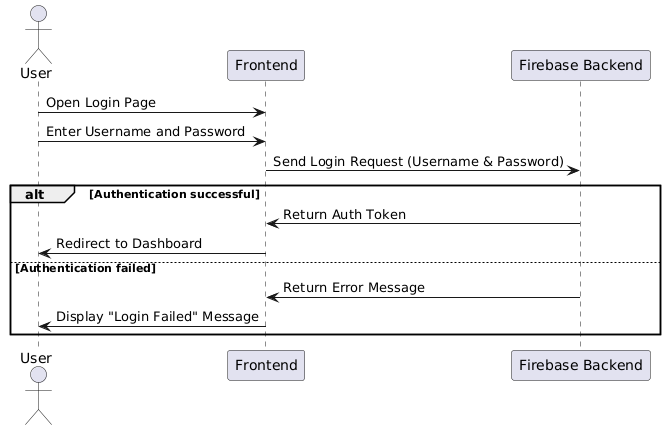
\includegraphics[width=\textwidth]{userlogin_seq.png} % Adjust the width to take the full text width, replace 'erd.jpeg' with your image file
 % Manually add the second caption below the table

\begin{center}
    \caption{User Login Sequence Diagram}
\end{center}
\end{figure}
\newpage
\vspace{1 cm} % Adjust this value to control the space before the background section

% Subsection title
\noindent
\subsubsection{User Signup}

\vspace{0.5cm} % Adjust this value to control the space before the background section
\noindent
\normalsize This diagram shows how the user can log in to the application. The user opens the mobile application, and the login page appears. The user clicks on the signup, and a signup page appears. The user enters their details to sign up. The system sends the details to the Firebase backend. If the user information is verified, the Firebase returns a success message, and the user can log into the application. But if the Firebase returns an error message then the system displays an error message to the user.
\vspace{0.5cm}
\begin{figure}[H]
    \centering
    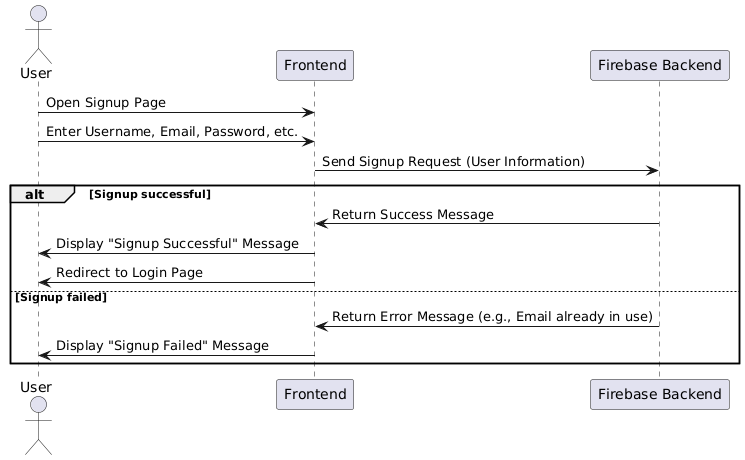
\includegraphics[width=\textwidth]{usersignup_seq.png} % Adjust the width to take the full text width, replace 'erd.jpeg' with your image file
 % Manually add the second caption below the table

\begin{center}
    \caption{User Signup Sequence Diagram}
\end{center}
\end{figure}

\newpage

\vspace{1 cm} % Adjust this value to control the space before the background section

% Subsection title
\noindent
\subsubsection{Add Expense}

\vspace{0.5cm} % Adjust this value to control the space before the background section
\noindent
\normalsize It depicts the process of adding expenses. The user clicks on the add button to add the expense by clicking on the category. The user can add expenses manually or by scanning receipts from photos. In both scenarios, the system
stores the data for further use by the Firebase backend.
\vspace{0.5cm}
\begin{figure}[H]
    \centering
    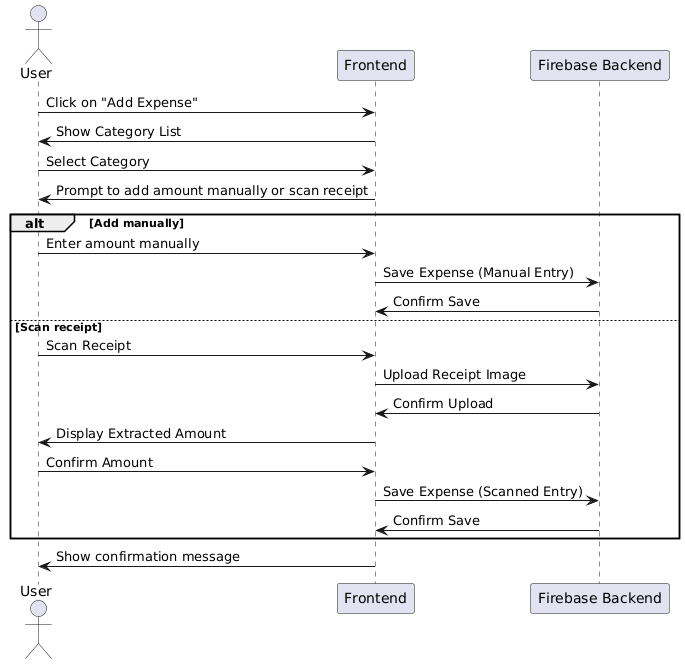
\includegraphics[width=\textwidth]{addexpense_seq.png} % Adjust the width to take the full text width, replace 'erd.jpeg' with your image file
 % Manually add the second caption below the table

\begin{center}
    \caption{Add Expense Sequence Diagram}
\end{center}
\end{figure}

\newpage

\vspace{1 cm} % Adjust this value to control the space before the background section

% Subsection title
\noindent
\subsubsection{Manage Budget}

\vspace{0.5cm} % Adjust this value to control the space before the background section
\noindent
\normalsize This diagram depicts the process of managing a budget. The user clicks on the manage button and requests budget suggestions from the Firebase backend. The Firebase then consults with an AI Model to provide recommendations based on the user's spending pattern. The AI Model sends back the calculated budget to the user, making it easy for the user to make financial decisions.
\vspace{0.5cm}
\begin{figure}[H]
    \centering
    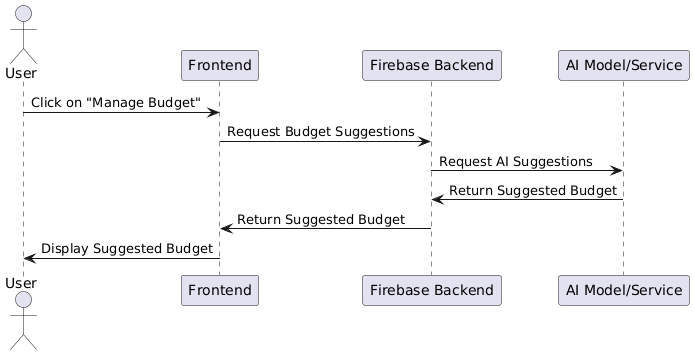
\includegraphics[width=\textwidth]{managebudget_seq.png} % Adjust the width to take the full text width, replace 'erd.jpeg' with your image file
 % Manually add the second caption below the table

\begin{center}
    \caption{Manage Budget Sequence Diagram}
\end{center}
\end{figure}
\newpage
\vspace{1 cm} % Adjust this value to control the space before the background section

% Subsection title
\noindent
\subsubsection{Next Month Budget}

\vspace{0.5cm} % Adjust this value to control the space before the background section
\noindent
\normalsize  This diagram shows the process of the "Next Month Budget". The user clicks on the "Budget Prediction" button. A request is generated to the Firebase backend. The backend then checks with an AI service. After the AI service calculates the next month's budget, it returns the predicted budget to the firebase, which sends it to the front end.
\vspace{0.5cm}
\begin{figure}[H]
    \centering
    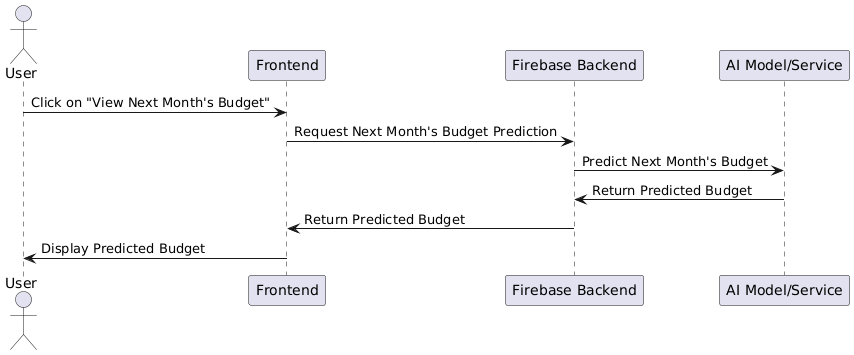
\includegraphics[width=\textwidth]{nextmonth_seq.png} % Adjust the width to take the full text width, replace 'erd.jpeg' with your image file
 % Manually add the second caption below the table

\begin{center}
    \caption{Next Month Budget Sequence Diagram}
\end{center}
\end{figure}
\newpage

\vspace{1 cm} % Adjust this value to control the space before the background section

% Subsection title
\noindent
\subsubsection{View Daily Life Products}

\vspace{0.5cm} % Adjust this value to control the space before the background section
\noindent
\normalsize The user clicks on View Daily Life Products, and the app requests the Firebase backend to provide product data. The backend then sends a request to an AI service to scrape e-commerce websites. The AI Model returns the data collected from these websites to the Firebase backend. The app then receives the data and displays it to the user.
\vspace{0.5cm}
\begin{figure}[H]
    \centering
    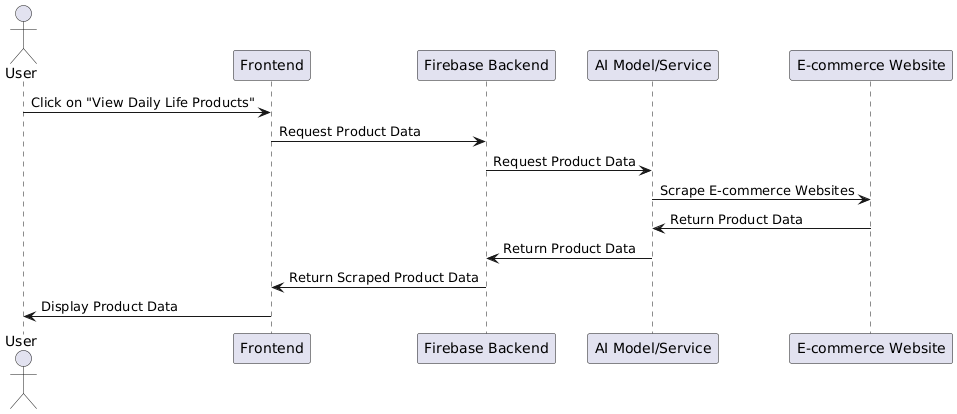
\includegraphics[width=\textwidth]{viewproduct_seq.png} % Adjust the width to take the full text width, replace 'erd.jpeg' with your image file
 % Manually add the second caption below the table

\begin{center}
    \caption{View Daily Life Products Sequence Diagram}
\end{center}
\end{figure}

\newpage

\vspace{1 cm} % Adjust this value to control the space before the background section

% Subsection title
\noindent
\subsubsection{Search Expense}

\vspace{0.5cm} % Adjust this value to control the space before the background section
\noindent
\normalsize It shows the process of search expenses. The user clicks on the search button and selects search by category or date options. After clicking the option, the app requests the Firebase to retrieve the relevant expense and sends back the data to the front end.
\vspace{0.5cm}
\begin{figure}[H]
    \centering
    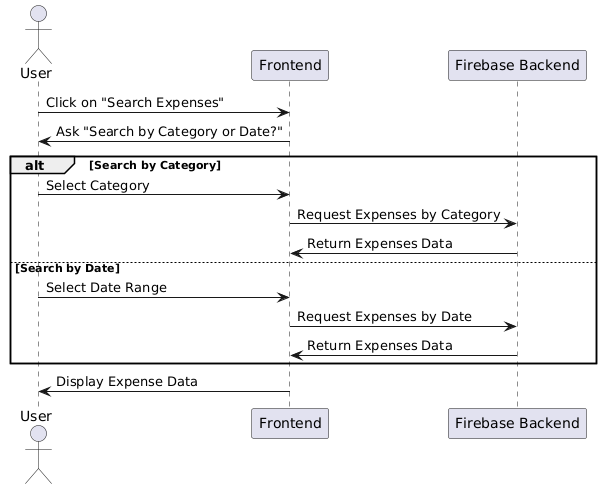
\includegraphics[width=\textwidth]{searchexpense.png} % Adjust the width to take the full text width, replace 'erd.jpeg' with your image file
 % Manually add the second caption below the table

\begin{center}
    \caption{Search Expense Sequence Diagram}
\end{center}
\end{figure}

\newpage
\vspace{1 cm} % Adjust this value to control the space before the background section

% Subsection title
\noindent
\subsubsection{Change Name}

\vspace{0.5cm} % Adjust this value to control the space before the background section
\noindent
\normalsize This sequence diagram shows how a user can change their name. The user navigates to the settings, selects the "change name" button and enters the new name. The front end sends the request to update, firebase updates and confirms the name change. The front end notifies the user that the name is updated. 
\vspace{0.5cm}
\begin{figure}[H]
    \centering
    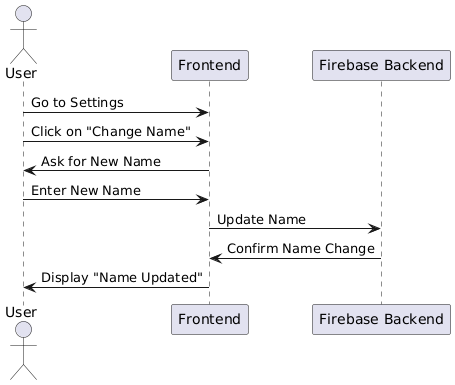
\includegraphics[width=\textwidth]{name_seq.png} % Adjust the width to take the full text width, replace 'erd.jpeg' with your image file
 % Manually add the second caption below the table

\begin{center}
    \caption{Change Name Sequence Diagram}
\end{center}
\end{figure}

\newpage
\vspace{1 cm} % Adjust this value to control the space before the background section

% Subsection title
\noindent
\subsubsection{Change Phone Number}

\vspace{0.5cm} % Adjust this value to control the space before the background section
\noindent
\normalsize This sequence diagram shows how a user can change their phone number. The user navigates to the settings, selects the "change number" button and enters the new name. The front end sends the request to update, firebase updates and confirms the name change. The front end notifies the user that the number is updated. 
\vspace{0.5cm}
\begin{figure}[H]
    \centering
    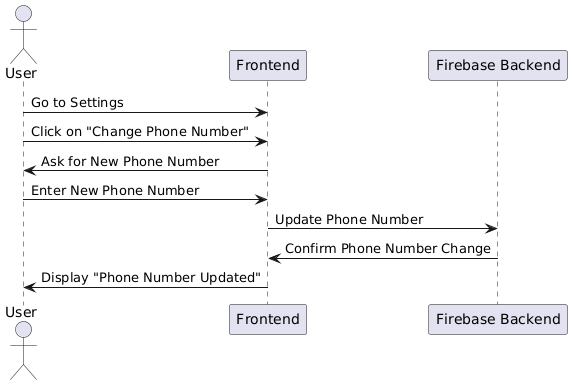
\includegraphics[width=\textwidth]{phonenum_seq.png} % Adjust the width to take the full text width, replace 'erd.jpeg' with your image file
 % Manually add the second caption below the table

\begin{center}
    \caption{Change Phone Number Sequence Diagram}
\end{center}
\end{figure}

\newpage
\vspace{1 cm} % Adjust this value to control the space before the background section

% Subsection title
\noindent
\subsubsection{Change Income amount}

\vspace{0.5cm} % Adjust this value to control the space before the background section
\noindent
\normalsize This process shows how the user changes the income amount. The user clicks the setting button and selects "change income amount".The user inputs the new income and the front end sends requests to the Firebase backend to update the amount entered. The firebase confirms the change to the front end and notifies the user.
\vspace{0.5cm}
\begin{figure}[H]
    \centering
    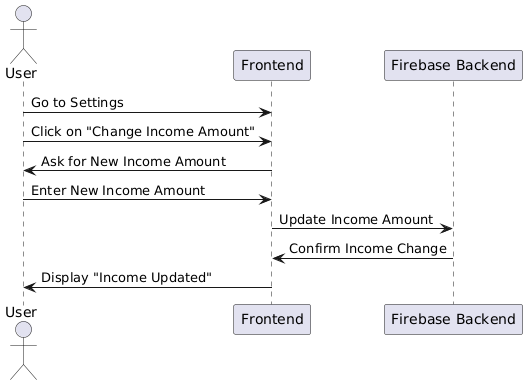
\includegraphics[width=\textwidth]{changeincome_seq.png} % Adjust the width to take the full text width, replace 'erd.jpeg' with your image file
 % Manually add the second caption below the table

\begin{center}
    \caption{Change Income amount Sequence Diagram}
\end{center}
\end{figure}
\newpage

\vspace{1 cm} % Adjust this value to control the space before the background section

% Subsection title
\noindent
\subsubsection{User Logout}

\vspace{0.5cm} % Adjust this value to control the space before the background section
\noindent
\normalsize In this diagram, the user wants to initiate a logout process. The user clicks on the button and selects the 'Logout' button. The front end sends an invalid token request to the Firebase backend. When it confirms that the session is invalidated, the user is redirected to the login page.

\begin{figure}[H]
    \centering
    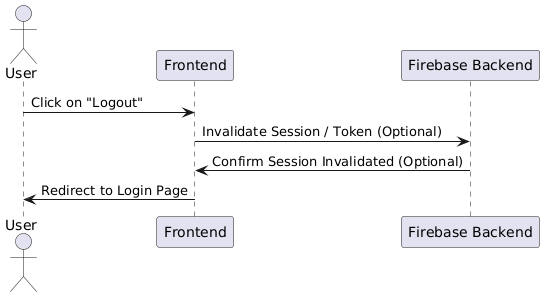
\includegraphics[width=\textwidth]{userlogout_seq.png} % Adjust the width to take the full text width, replace 'erd.jpeg' with your image file
 % Manually add the second caption below the table
 \begin{center}
    \caption{User Logout Sequence Diagram}
\end{center}
\end{figure}


\newpage

\vspace{1 cm} % Adjust this value to control the space before the background section

% Subsection title
\noindent
\subsubsection{Admin Sequence Diagram}

\vspace{0.5cm} % Adjust this value to control the space before the background section
\noindent
\normalsize
\begin{figure}[H]
    \centering
    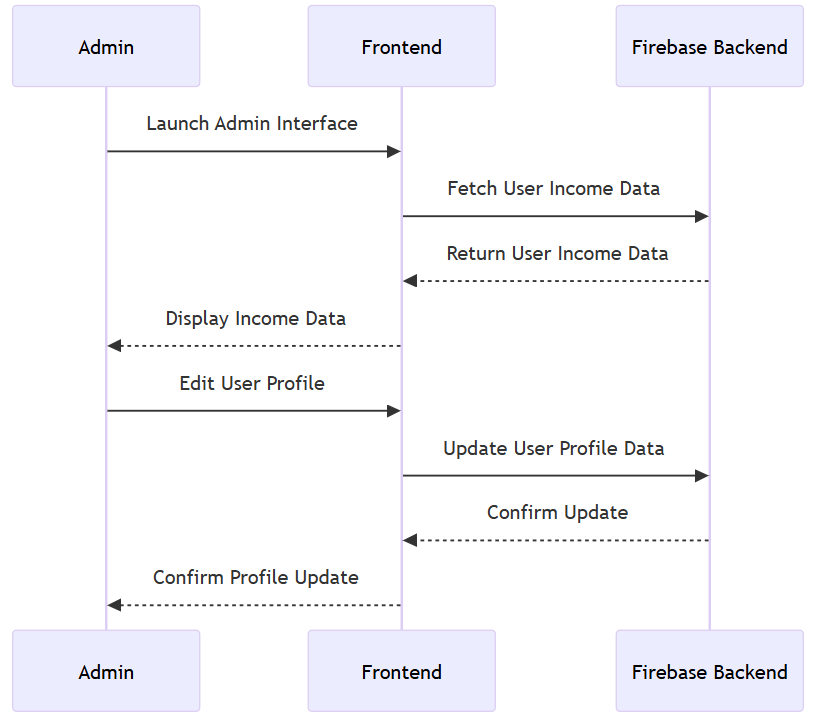
\includegraphics[width=\textwidth]{admin_seq.PNG} % Adjust the width to take the full text width, replace 'erd.jpeg' with your image file
 % Manually add the second caption below the table

\begin{center}
    \caption{Admin Sequence Diagram Sequence Diagram}
\end{center}
\end{figure}
\newpage

\vspace{1 cm} % Adjust this value to control the space before the background section

% Subsection title
\noindent
\subsubsection{Admin Login}

\vspace{0.5cm} % Adjust this value to control the space before the background section
\noindent
\normalsize It shows the process how an admin log into the centralized system. The admin enters its login credentials on the frontend interface. The front end send requests to the Firebase backend to verify the credentials entered by the admin. If the Firebase backend returns the authorization token, the admin can proceed to the dashboard. On the other hand, if the Firebase backend returns an error message, the front end displays a login failed message.
\vspace{1 cm}
\begin{figure}[H]
    \centering
    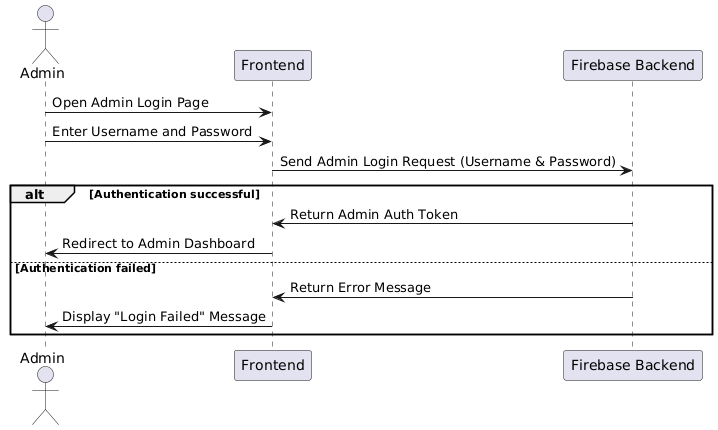
\includegraphics[width=\textwidth]{admin_login.png} % Adjust the width to take the full text width, replace 'erd.jpeg' with your image file
 % Manually add the second caption below the table

\begin{center}
    \caption{Admin Login Sequence Diagram}
\end{center}
\end{figure}
\newpage

\vspace{1 cm} % Adjust this value to control the space before the background section

% Subsection title
\noindent
\subsubsection{View User Details}

\vspace{0.5cm} % Adjust this value to control the space before the background section
\noindent
\normalsize This sequence diagram shows how the admin views user  details. After logging in through the credentials, then open the user detail page. The frontend sends a request to the database to fetch the user  data, return the user's  data to the front-end and display it to the admin.
\vspace{1 cm}
\begin{figure}[H]
    \centering
    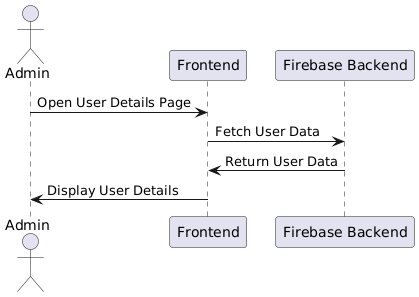
\includegraphics[width=\textwidth]{adminuserdetail_seq.png} % Adjust the width to take the full text width, replace 'erd.jpeg' with your image file
 % Manually add the second caption below the table

\begin{center}
    \caption{View User Details Sequence Diagram}
\end{center}
\end{figure}
\newpage
\vspace{1 cm} % Adjust this value to control the space before the background section

% Subsection title
\noindent
\subsection{Mobile Application}
\vspace{0.5cm} % Adjust this value to control the space before the background section
\noindent
\normalsize
Our Mobile Application consists of different features and Modules. Some screenshots of those features are given below:
\subsubsection{Login}
\vspace{1 cm}
\begin{figure}[H]
    \centering
    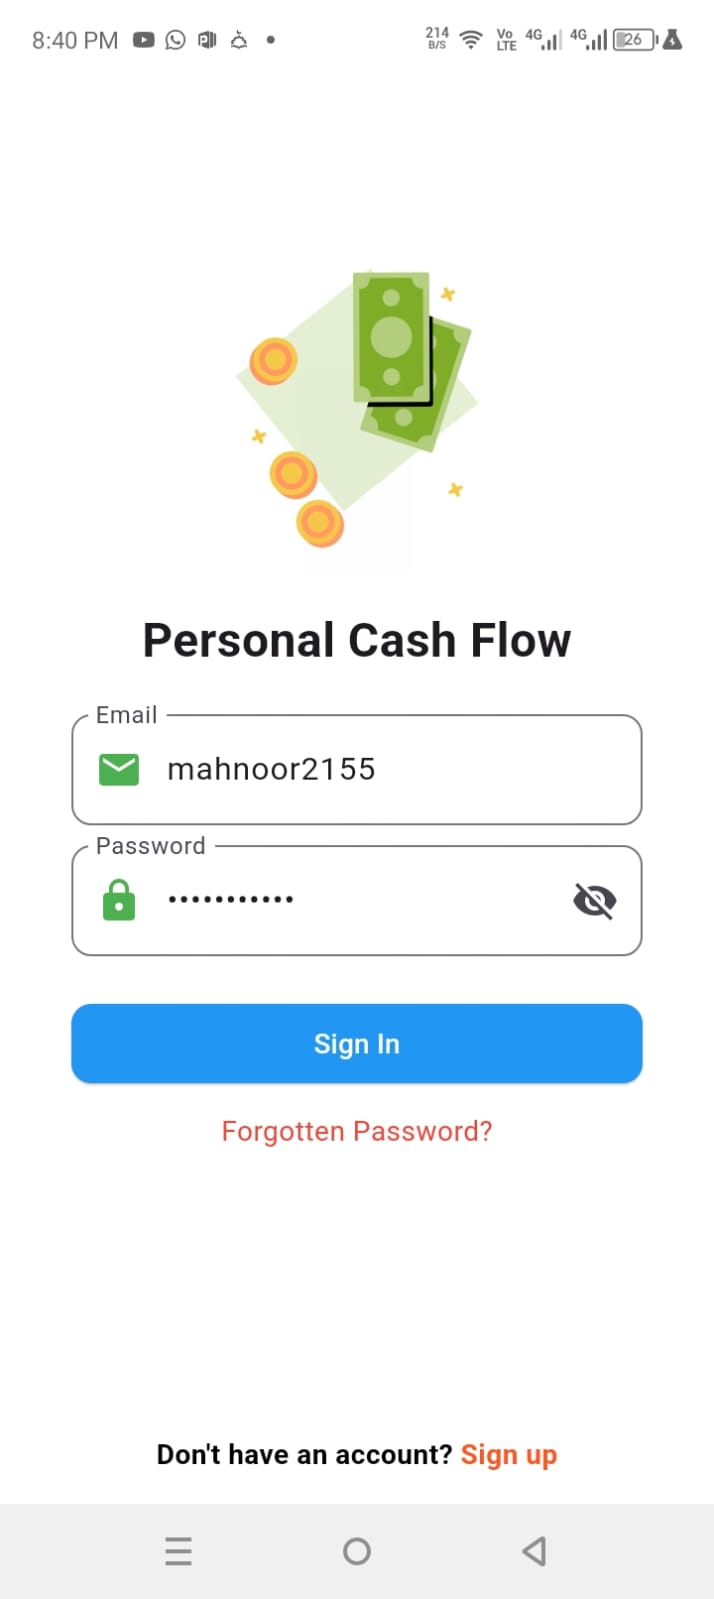
\includegraphics[height=15cm]{login.jpeg} % Adjust the height value as needed
    \caption{User Login}
\end{figure}
\newpage
\subsubsection{Signup}
\vspace{1 cm}
\begin{figure}[H]
    \centering
    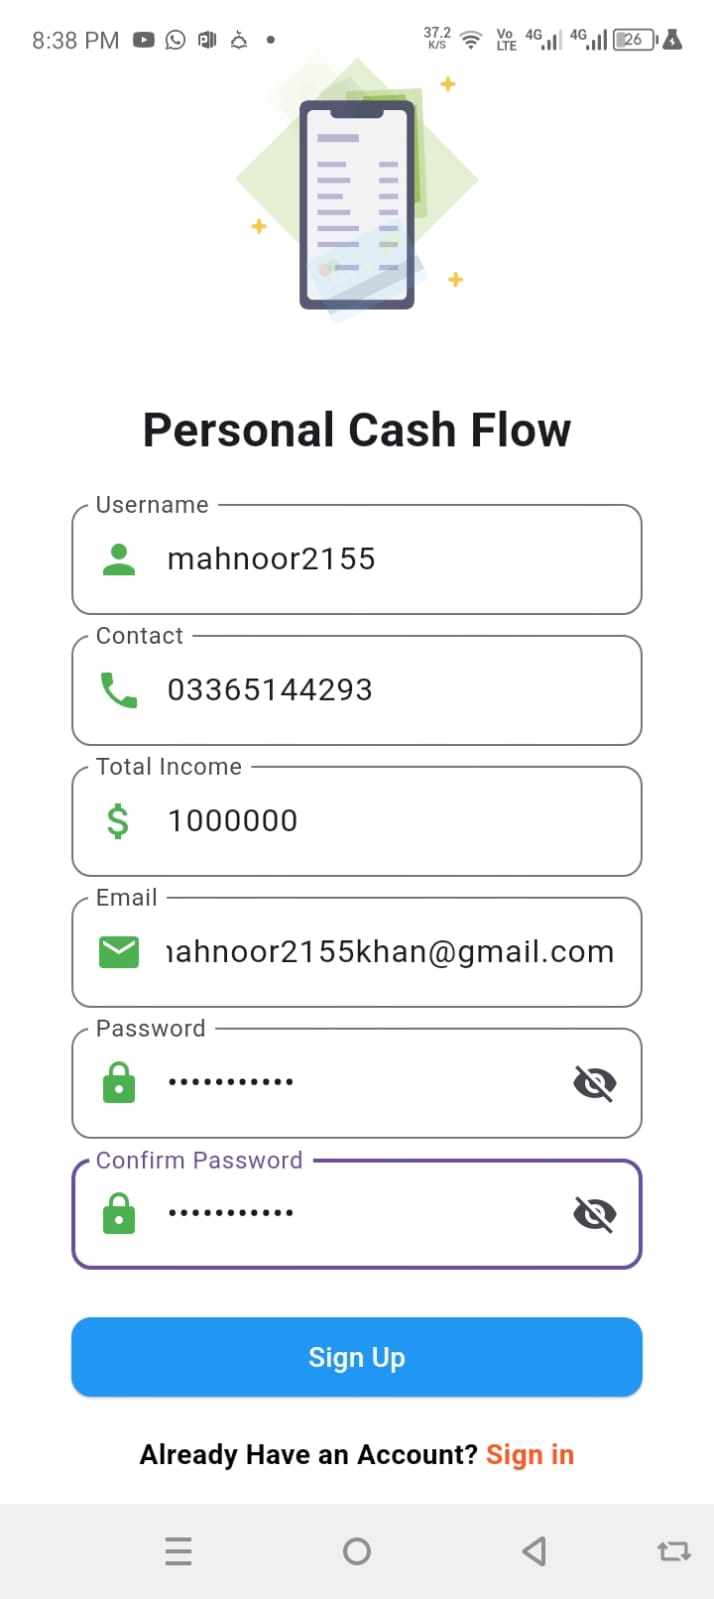
\includegraphics[height=20cm]{signup.jpeg} % Adjust the height value as needed
    \caption{User Signup}
\end{figure}

\newpage
\subsubsection{Dashboard}
\vspace{1 cm}
\begin{figure}[H]
    \centering
    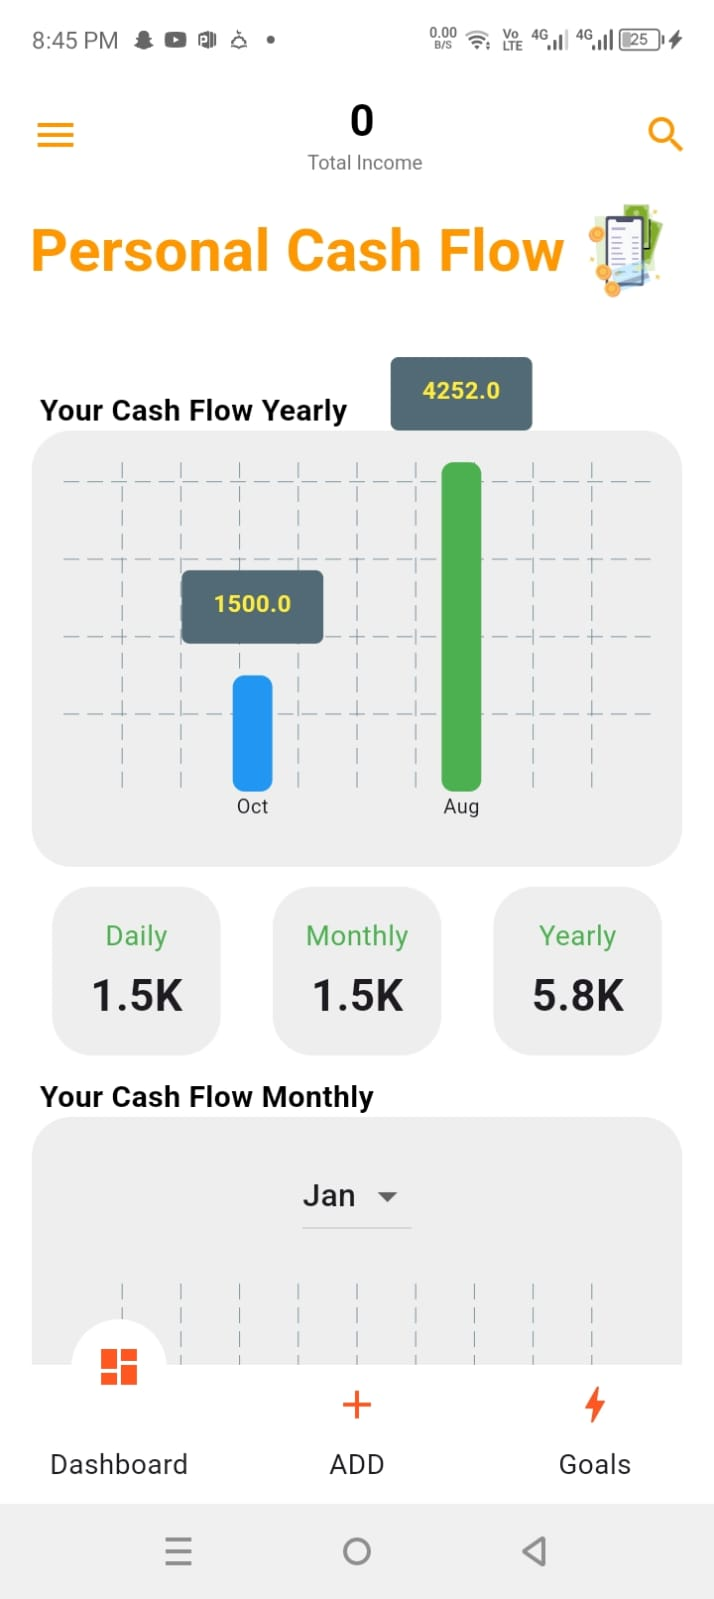
\includegraphics[height=20cm]{dashboard.jpeg} % Adjust the height value as needed
    \caption{Dashboard}
\end{figure}

\newpage
\subsubsection{Navigator Bar}
\vspace{1 cm}
\begin{figure}[H]
    \centering
    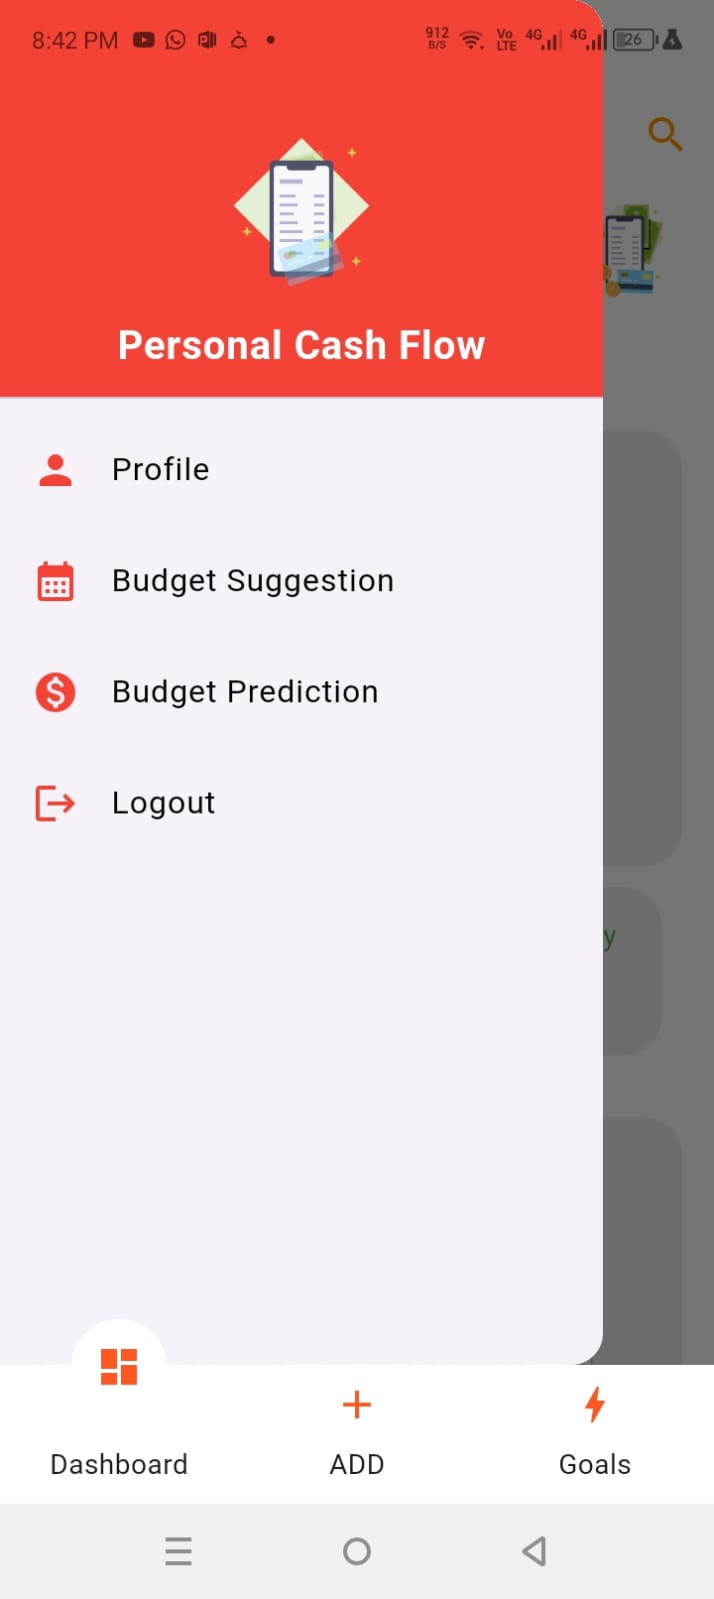
\includegraphics[height=20cm]{sidemenu.jpeg} % Adjust the height value as needed
    \caption{Navigator Bar}
\end{figure}

\newpage
\subsubsection{Add Expense}
\vspace{1 cm}
\begin{figure}[H]
    \centering
    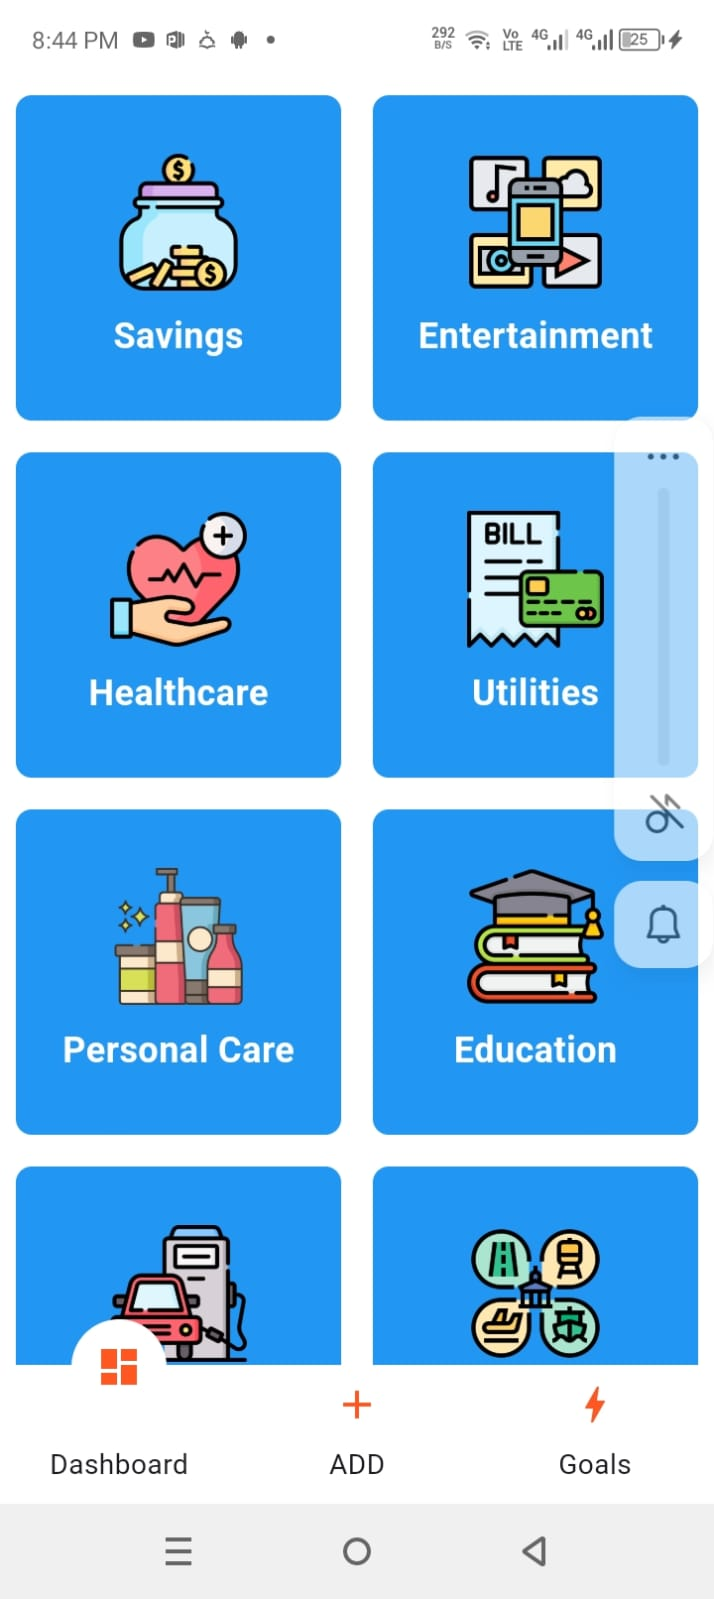
\includegraphics[height=20cm]{addexpense.jpeg} % Adjust the height value as needed
    \caption{Add Expense}
\end{figure}

\newpage
\subsubsection{Add Expense Manually}
\vspace{1 cm}
\begin{figure}[H]
    \centering
    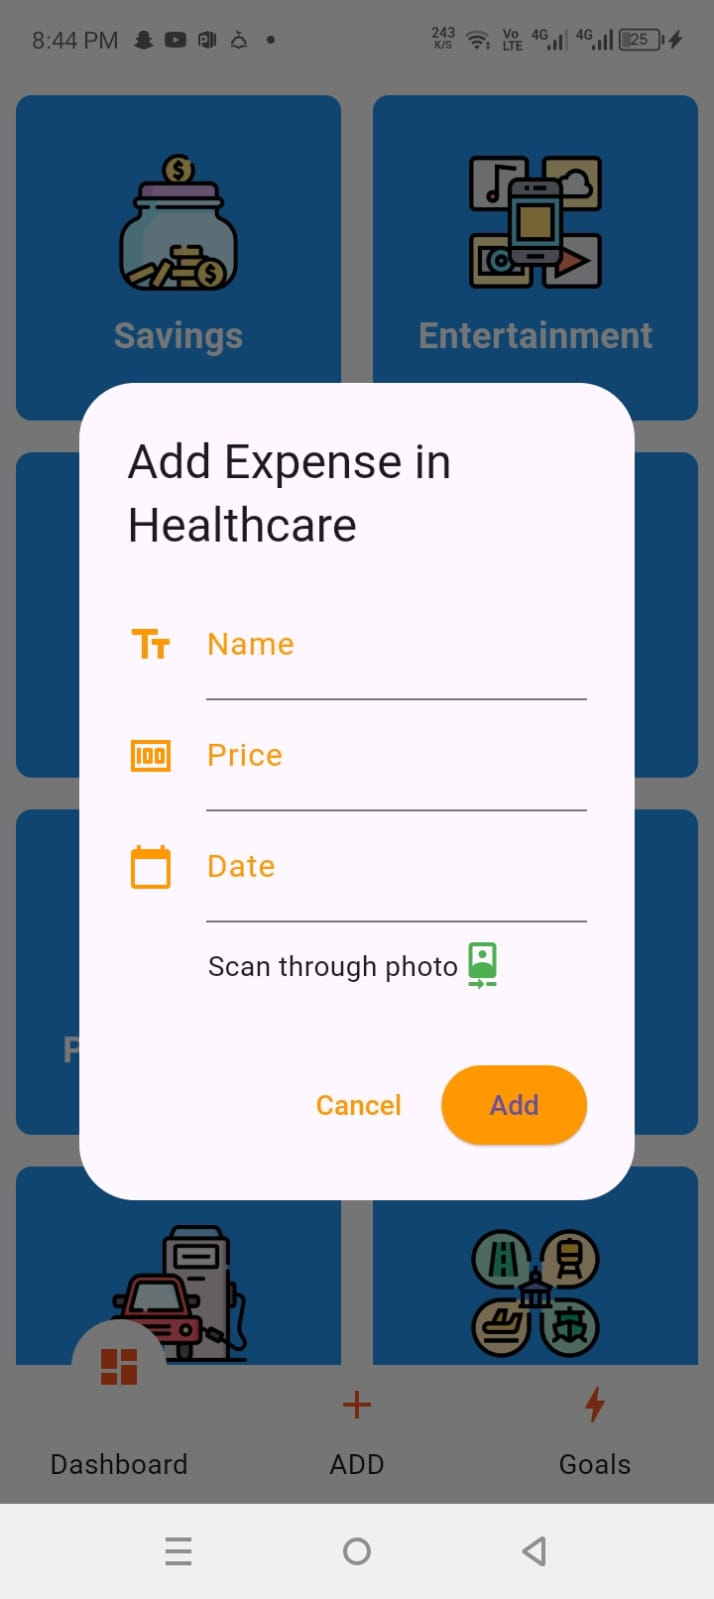
\includegraphics[height=20cm]{addexpensemanually.jpeg} % Adjust the height value as needed
    \caption{Add Expense Manually}
\end{figure}

\newpage
\subsubsection{Scan receipt through photos}
\vspace{1 cm}
\begin{figure}[H]
    \centering
    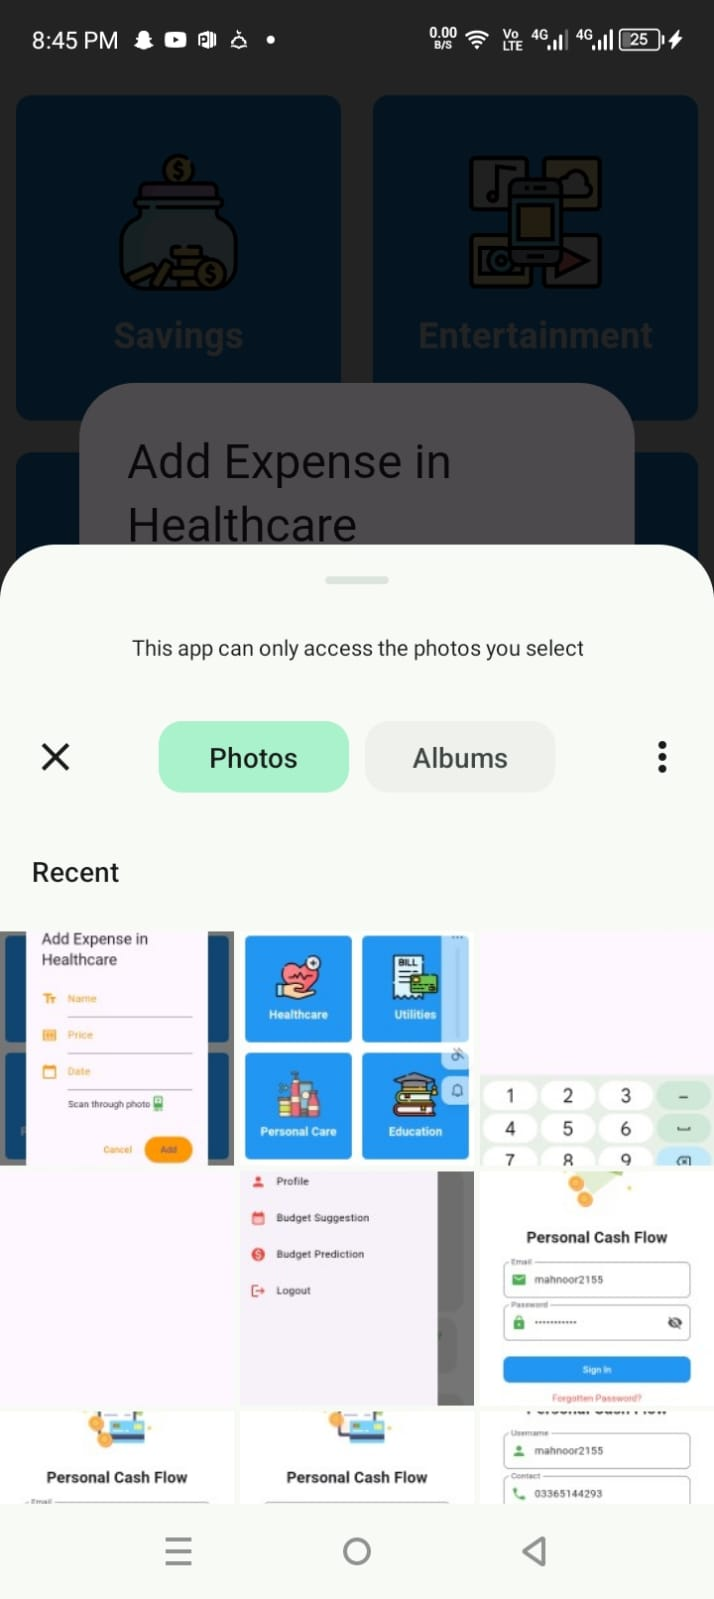
\includegraphics[height=20cm]{selectfromgallery.jpeg} % Adjust the height value as needed
    \caption{Scan receipt through photos}
\end{figure}


\newpage
\subsubsection{Set Goals}
\vspace{1 cm}
\begin{figure}[H]
    \centering
    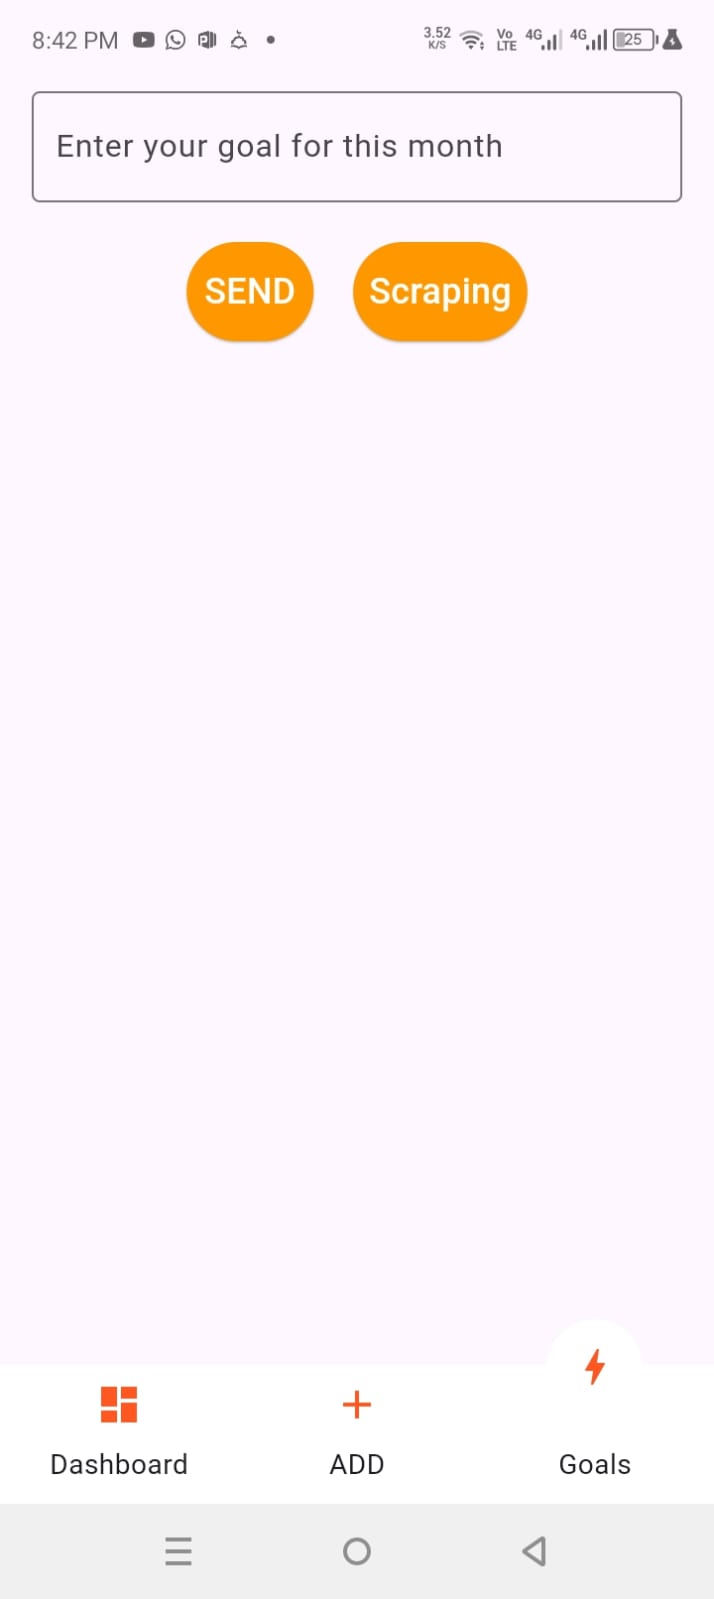
\includegraphics[height=20cm]{Goals.jpeg} % Adjust the height value as needed
    \caption{Set Goals}
\end{figure}

\newpage
\subsubsection{Search Expense By Date}
\vspace{1 cm}
\begin{figure}[H]
    \centering
    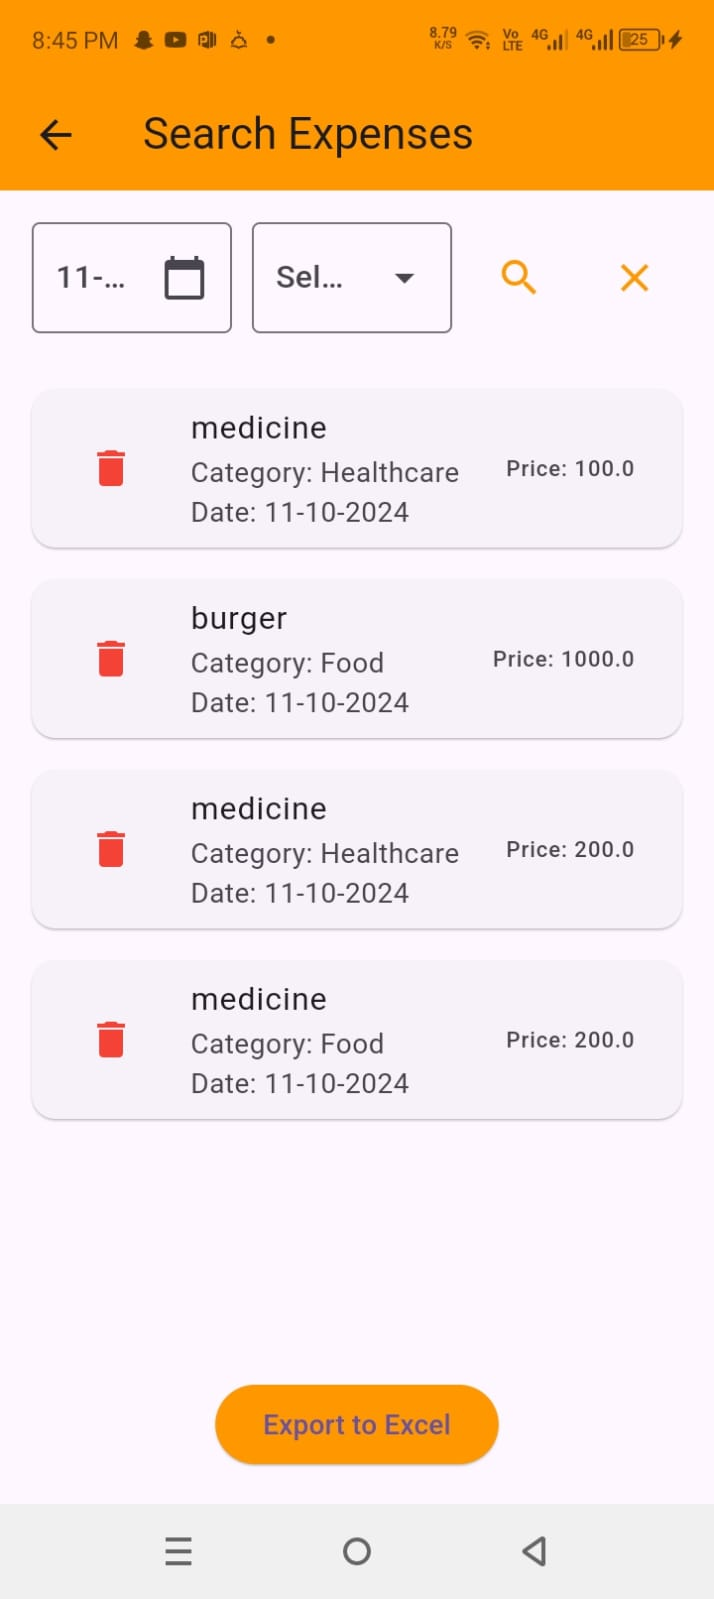
\includegraphics[height=20cm]{searchexpenses.jpeg} % Adjust the height value as needed
    \caption{Search Expenses By Date}
\end{figure}

\newpage
\subsubsection{Search Expense By Category}
\vspace{1 cm}
\begin{figure}[H]
    \centering
    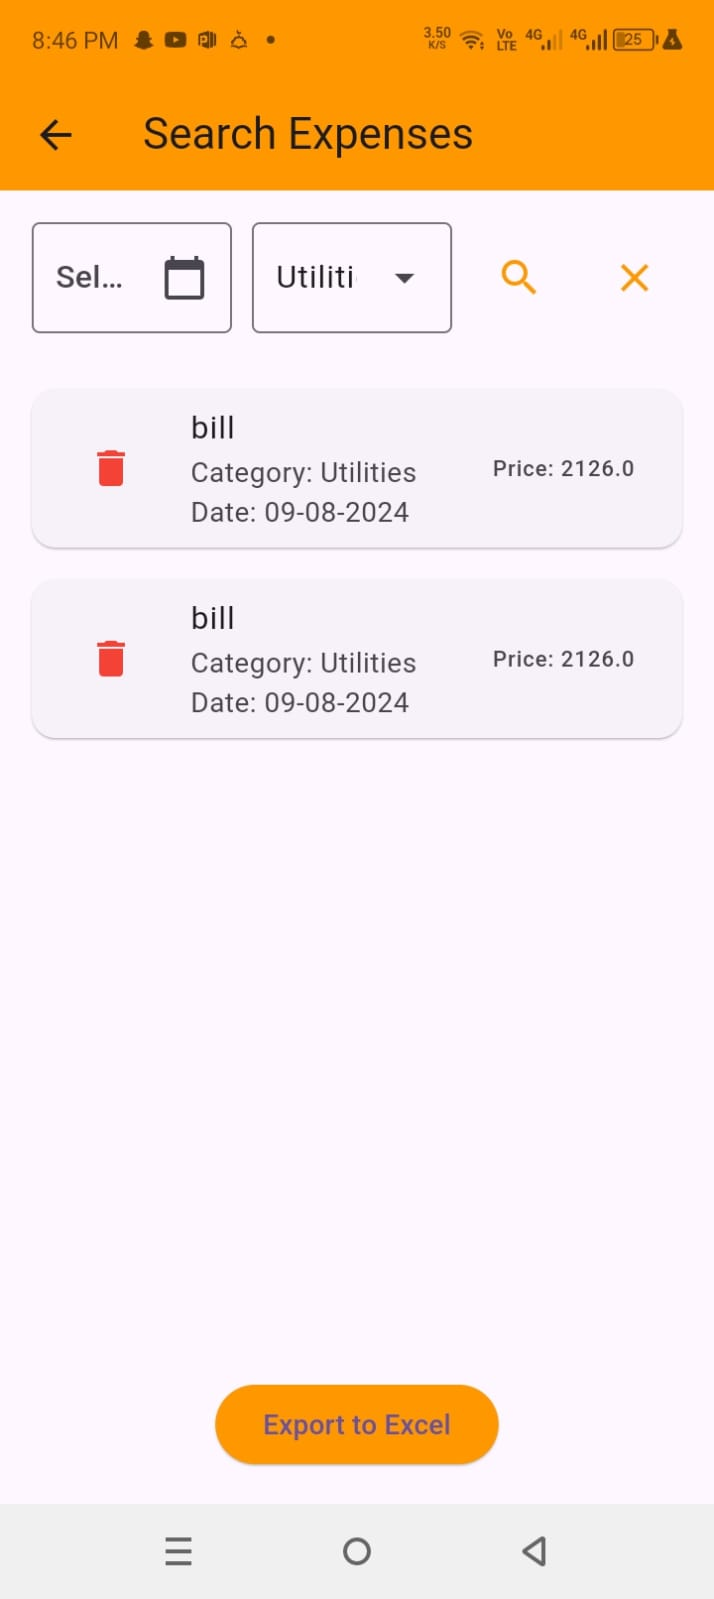
\includegraphics[height=20cm]{searchdate.jpeg} % Adjust the height value as needed
    \caption{Search Expenses By Category}
\end{figure}

\newpage
\subsubsection{Admin Login}
\vspace{1 cm}
\begin{figure}[H]
    \centering
    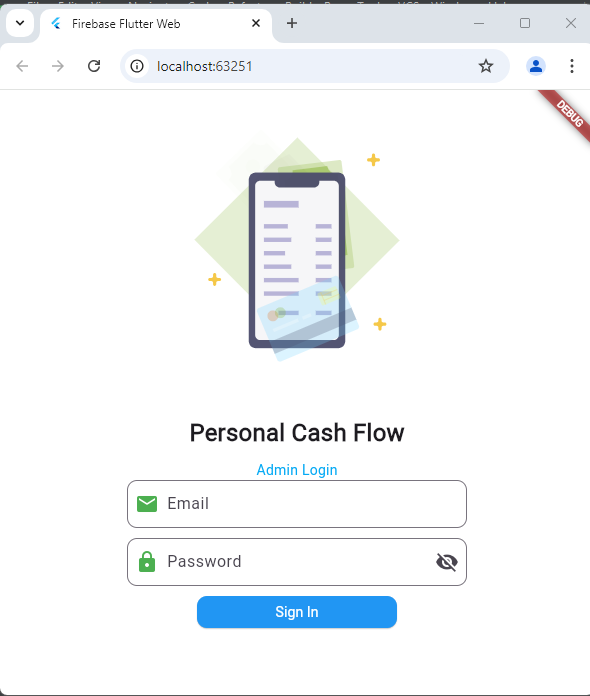
\includegraphics[width=15cm,height=18cm]{adminlogin.png} % Adjust the height value as needed
    \caption{Admin Login}
\end{figure}

\newpage
\subsubsection{Admin Dasboard}
\vspace{1 cm}
\begin{figure}[H]
    \centering
    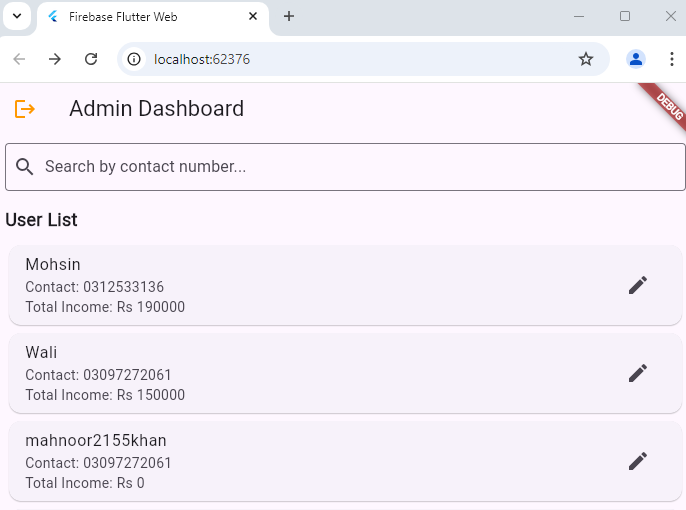
\includegraphics[width=15cm,height=18cm]{admindashboard.png} % Adjust the height value as needed
    \caption{Admin Dashboard}
\end{figure}

\newpage

\vspace*{1.5cm} % Adjust this value to control the vertical position of the chapter title

% Chapter title
\noindent
\LARGE \textbf{Chapter 5}

\vspace{1 cm}

% Section title
\noindent
\section{System Implementation}

\vspace{0.5cm} % Adjust this value to control the space between the title and the content

% Introduction content
\noindent
\normalsize The process of bringing an idea from concept to reality is called implementation. A technical specification or method is realized as a program, software component, or other computer system by programming and de-ployment, which is known as system implementation.Implementation is the process of moving an idea from concept to reality. The System implementation is a realization of a technical specification or algorithm as a program, software component, or other computer system through programming and deployment.\cite{anitha2016easy}
\vspace{0.5cm} % Adjust this value to control the space between the title and the content

% Introduction content
\noindent
\subsection{System Implementation}
\vspace{0.5cm} % Adjust this value to control the space between the title and the content

% Introduction content
\noindent
\normalsize In this chapter we will discuss how the system will be implemented in real which involves structure of the system, main components of the system and tools and technologies used for the system to be fully implemented. 
\vspace{0.5cm} % Adjust this value to control the space between the title and the content

% Introduction content
\noindent
\subsection{System Architecture}
\vspace{0.5cm} % Adjust this value to control the space between the title and the content

% Introduction content
\noindent
\normalsize The architecture of this system is designed in a way to provide an easy and user-friendly expense-tracking solution. The frontend of this project is created through Flutter which utilizes cutting-edge technologies and a backend system to handle the user data and user authentication. All the user data is secured in the Firebase database. The centralized admin panel built through Flutter web to  views user income details. The system architecture of the personal cash flow navigator is designed to provide a robust and scalable platform for expense management.\cite{bozkus2009analytical}
On the front end, Personal Cash Flow Navigator utilizes Flutter to create a dynamic and responsive user interface, offering a seamless experience for users. 
The firebase serves as the primary database for Personal Cash Flow Navigator providing a scalable and efficient environment for storing and retrieving data, handling user authentication and handling user data. It ensures the offer of real-time data to the users.
The machine learning algorithm analyzes user behaviour and provides tailored suggestions and predictions for the next month. It enhances the functionality and user experience of the platform.
Overall, the system architecture of Personal Cash Flow Navigator is designed to be modular, scalable, and extensible, enabling the platform to accommodate future growth and changes in user demand while delivering a seamless and responsive expense management experience to users across Pakistan.\cite{khandelwal2022developing}




\vspace{0.5cm} % Adjust this value to control the space between the title and the content

% Introduction content
\noindent
\subsection{Tools and technologies}
\vspace{0.5cm} % Adjust this value to control the space between the title and the content

% Introduction content
\noindent
\normalsize The table highlights the tools and technologies utilized in creating a mobile app for Personal Cash Flow Navigator. Latex is used for project documentation, Visual Paradigm for system diagrams,
Draw.io for user interaction diagrams, and Android Studio for coding. These tools
collectively enable efficient development and robust functionality in the mobile app.
\vspace{0.5cm}
\begin{table}[h!]
\centering
\resizebox{\textwidth}{!}{  % Resizes the table to fit the text width
\begin{tabular}{|l|l|}
\hline
\textbf{Tools/Technology}       & Purpose \\ \hline
\textbf{Flutter} & Frontend development of mobile application. \\ \hline
\textbf{Firebase}      & Backend services for user authentication and database storage \\ \hline
\textbf{Dart}              & Programming language used for Flutter development \\ \hline
\textbf{Python}    & Used for developing machine learning algorithms and backend logic \\ \hline
\textbf{Admin Panel(Flutter Web)}             & View user income details.\\ \hline
\end{tabular}
}

\begin{center}
    \caption{Tools and Technology}
\end{center}
\vspace{0.5 cm}
\end{table}
\newpage


% Chapter title
\noindent
\LARGE \textbf{Chapter 6}

\vspace{1 cm}

% Section title
\noindent
\section{System Testing and Evaluation}

\vspace{0.5cm} % Adjust this value to control the space between the title and the content

% Introduction content
\noindent
\normalsize Testing is a process, in which we put the system under some test to increase the system functionality and reduce the risk of potential errors. It makes sure that all the errors are removed before the release of the system. The proposed system is evaluated to check if it behaves as planned and the system is reliable and user-friendly. It increases reliability and maximizes user satisfaction by identifying defects and solving them before the system's deployment.\cite{chandini2019online}
\vspace{0.5cm} % Adjust this value to control the space between the title and the content

% Introduction content
\noindent
\subsection{Functional Testing}
\vspace{0.5cm} % Adjust this value to control the space between the title and the content

% Introduction content
\noindent
\normalsize The functional testing ensures that the system software works as intended and that all functional requirements are completed. It checks that every software feature works according to the instructions.
\vspace{0.5cm} % Adjust this value to control the space between the title and the content

% Introduction content
\noindent
\subsubsection{Unit Testing}
\vspace{0.5cm} % Adjust this value to control the space between the title and the content 

% Introduction content
\noindent
\normalsize It is a type of Testing where each module is tested independently, to ensure it works properly. Every module is called a unit. We perform this test to make sure that any issues found within a unit are identified and solved before integrating them into the other parts.
\vspace{0.5cm} % Adjust this value to control the space between the title and the content

% Introduction content
\noindent
\subsubsection{Integration Testing}
\vspace{0.5cm} % Adjust this value to control the space between the title and the content 

% Introduction content
\noindent
\normalsize In Integration testing, All the modules are combined so that they can be tested as a single system. It is checked whether or not the units combined function properly then they are integrated.\cite{chianglin2008personal} First tested the units through unit testing then the units are tested when integrated to check its working correctly or not. Our proposed system was integrated after the units were cleared, the integration of modules that are User authentication, Budget Prediction and suggestions was done and integration testing was done to make sure that they are working properly.\cite{french2021personal}
\vspace{0.5cm} % Adjust this value to control the space between the title and the content

% Introduction content
\noindent
\subsubsection{System Testing}
\vspace{0.5cm} % Adjust this value to control the space between the title and the content 


% Introduction content
\noindent
\normalsize First tested the units through unit testing then the system is tested as a whole to check its working correctly or not. After integration testing is done the system should be tested to see whether it works correctly as a system or not. Our proposed system was tested as a single system after the integration was done. All the modules were combined and run as a single system to perform the task. After the successful test, the system is ready for deployment.\\

\vspace{0.5 cm}
% Section title
\noindent
\subsection{Non Functional Requirements}
\vspace{0.5cm} % Adjust this value to control the space between the title and the content

% Introduction content
\noindent
\normalsize This section ensures that all of the non-functional requirements of the proposed system are met.
\vspace{0.5cm} % Adjust this value to control the space between the title and the content

% Introduction content
\noindent
\subsubsection{Performance Testing}
\vspace{0.5cm} % Adjust this value to control the space between the title and the content

% Introduction content
\noindent
\normalsize We evaluated the system's total response time. like how long it takes for our application to add expense, get budget prediction or suggestion. The response time has been kept as short as possible. Performance testing led us to the conclusion that our system is responsive all around.\cite{bozkus2009analytical}
\vspace{0.5cm}

% Introduction content
\noindent
\subsubsection{Acceptance Testing}
\vspace{0.5cm} % Adjust this value to control the space between the title and the content

% Introduction content
\noindent
\normalsize We verified that the system's major requirements are met. We verified whether or not all of the functional requirements from the objective section had been met.

\vspace{1 cm}
% Section title
\noindent
\subsection{Test Cases}

\vspace{0.5cm} % Adjust this value to control the space between the title and the content

% Introduction content
\noindent
\normalsize The test case can be defined as a scenario in which functionality is approximated across a variety of activities or conditions to confirm the desired result. Test cases are different types of tests that are used to have every kind of scenario possible for the proposed system. They can be used on any kind of system whether the system is automated or manual. In this phase, we verified the system's functioning and accuracy. The system and its parts are put to the test with various inputs, and the system's output is compared to the intended output.
\newpage
\vspace{1 cm}

% Introduction content
\noindent
\subsubsection{User Login with Valid Credentials}
\begin{table}[h!]
\centering
\resizebox{\textwidth}{!}{  % Resizes the table to fit the text width
\begin{tabular}{|l|l|}
\hline
\textbf{Test Case ID}       & TC-001 \\ \hline
\textbf{Testable Functionality} & User Login with Valid Credentials \\ \hline
\textbf{Initial State}      & App is open, user is at the login screen \\ \hline
\textbf{Input}              & Valid email and password \\ \hline
\textbf{Expected Result}    & The user should be logged in successfully and redirected to the dashboard \\ \hline
\textbf{Result}             & Pass\\ \hline
\textbf{Status}             & Pass/Fail \\ \hline
\end{tabular}
}

\begin{center}
    \caption{User Login with Valid Credentials: Test Case 1}
\end{center}
\vspace{0.5 cm}
\end{table}
% Introduction content
\noindent
\subsubsection{User Login with Invalid Credentials}
\begin{table}[h!]
\centering
\resizebox{\textwidth}{!}{  % Resizes the table to fit the text width
\begin{tabular}{|l|l|}
\hline
\textbf{Test Case ID}       & TC-002 \\ \hline
\textbf{Testable Functionality} & User Login with Invalid Credentials \\ \hline
\textbf{Initial State}      & App is open, user is at the login screen \\ \hline
\textbf{Input}              & Invalid email or password \\ \hline
\textbf{Expected Result}    & Error message should be displayed, and the user should remain on the login screen \\ \hline
\textbf{Result}             & Pass\\ \hline
\textbf{Status}             & Pass/Fail \\ \hline
\end{tabular}
}

\begin{center}
    \caption{User Login with Invalid Credentials: Test Case 2}
\end{center}

\vspace{0.5 cm}
\end{table}
% Introduction content
\noindent
\subsubsection{User Sign up}
\begin{table}[h!]
\centering
\resizebox{\textwidth}{!}{  % Resizes the table to fit the text width
\begin{tabular}{|l|l|}
\hline
\textbf{Test Case ID}       & TC-003 \\ \hline
\textbf{Testable Functionality} & User Sign up \\ \hline
\textbf{Initial State}      & App is open, user is on the sign up screen \\ \hline
\textbf{Input}              & Valid email, password, and required information \\ \hline
\textbf{Expected Result}    & The user should be successfully registered and redirected to the login screen \\ \hline
\textbf{Result}             & Pass \\ \hline
\textbf{Status}             & Pass/Fail \\ \hline
\end{tabular}
}

\begin{center}
    \caption{User Sign up: Test Case 3}
\end{center}

\vspace{0.5 cm}
\end{table}
\newpage
% Introduction content
\noindent
\subsubsection{Existing User Sign up}
\begin{table}[h!]
\centering
\resizebox{\textwidth}{!}{  % Resize the table to fit the page width
\begin{tabular}{|l|l|}
\hline
\textbf{Test Case ID}       & TC-004 \\ \hline
\textbf{Testable Functionality} & Existing User Signup \\ \hline
\textbf{Initial State}      & App is open, user is at the signup screen, user account already exists \\ \hline
\textbf{Input}              & Enter existing email and password in the Signup page \\ \hline
\textbf{Expected Result}    & The system should display an error message indicating that the user is already registered, and prompt them to log in instead. \\ \hline
\textbf{Result}             & Pass \\ \hline
\textbf{Status}             & Pass/Fail \\ \hline
\end{tabular}
}

\begin{center}
    \caption{Existing User Signup : Test Case 4}
\end{center}
\newpage

\vspace{0.5 cm}
\end{table}
% Introduction content
\noindent
\subsubsection{Add New Expense Manually}
\begin{table}[h!]
\centering
\resizebox{\textwidth}{!}{  % Resizes the table to fit the text width
\begin{tabular}{|l|l|}
\hline
\textbf{Test Case ID}       & TC-005 \\ \hline
\textbf{Testable Functionality} & Add New Expense Manually \\ \hline
\textbf{Initial State}      & App is open and user clicks on the add button. \\ \hline
\textbf{Input}              & Valid email, password, and required information \\ \hline
\textbf{Expected Result}    & The user should be successfully registered and redirected to the login screen \\ \hline
\textbf{Result}             & Pass\\ \hline
\textbf{Status}             & Pass/Fail \\ \hline
\end{tabular}
}

\begin{center}
    \caption{Add New Expense Manually: Test Case 5}
\end{center}

\vspace{0.5 cm}
\end{table}
% Introduction content
\noindent
\subsubsection{Add New Expense Through Scan Receipt}
\begin{table}[h!]
\centering
\resizebox{\textwidth}{!}{  % Resizes the table to fit the text width
\begin{tabular}{|l|l|}
\hline
\textbf{Test Case ID}       & TC-006 \\ \hline
\textbf{Testable Functionality} & Add New Expense Through Scan Receipt \\ \hline
\textbf{Initial State}      & User is logged in, and the device has photos available in the gallery \\ \hline
\textbf{Input}              & 1. Navigate to the "Add Expense" screen. \newline 2. Select "Scan Receipt". \newline 3. Choose an image from the photo gallery. \\ \hline
\textbf{Expected Result}    & The system should extract the receipt details from the selected image and populate the expense fields automatically. \\ \hline
\textbf{Result}             & Pass\\ \hline
\textbf{Status}             & Pass/Fail \\ \hline
\end{tabular}
}

\begin{center}
    \caption{Add New Expense Through Scan Receipt: Test Case 6}
\end{center}

\vspace{0.5 cm}
\end{table}

% Introduction content
\noindent
\subsubsection{Search Expenses by Date}
\newpage
\begin{table}[h!]
\centering
\resizebox{\textwidth}{!}{  % Resizes the table to fit the text width
\begin{tabular}{|l|l|}
\hline
\textbf{Test Case ID}       & TC-007 \\ \hline
\textbf{Testable Functionality} & Search Expenses by Date \\ \hline
\textbf{Initial State}      & User is logged in and at the "Search Expenses" screen \\ \hline
\textbf{Input}              & Enter a date \\ \hline
\textbf{Expected Result}    & Expenses within the selected date should be displayed \\ \hline
\textbf{Result}             & Pass\\ \hline
\textbf{Status}             & Pass/Fail \\ \hline
\end{tabular}
}

\begin{center}
    \caption{Search Expenses by Date: Test Case 7}
\end{center}

\vspace{0.5 cm}
\end{table}
% Introduction content
\noindent
\subsubsection{Search Expenses by Category}
\begin{table}[h!]
\centering
\resizebox{\textwidth}{!}{  % Resizes the table to fit the text width
\begin{tabular}{|l|l|}
\hline
\textbf{Test Case ID}       & TC-008 \\ \hline
\textbf{Testable Functionality} & Search Expenses by Category \\ \hline
\textbf{Initial State}      & User is logged in and at the "Search Expenses" screen \\ \hline
\textbf{Input}              & Select a category. \\ \hline
\textbf{Expected Result}    & All expenses within the selected category should be displayed \\ \hline
\textbf{Result}             & Pass\\ \hline
\textbf{Status}             & Pass/Fail \\ \hline
\end{tabular}
}

\begin{center}
    \caption{Search Expenses by Category: Test Case 8}
\end{center}
\vspace{0.5 cm}
\end{table}
% Introduction content
\noindent
\subsubsection{View Expense Graphs}
\begin{table}[h!]
\centering
\resizebox{\textwidth}{!}{  % Resizes the table to fit the text width
\begin{tabular}{|l|l|}
\hline
\textbf{Test Case ID}       & TC-009 \\ \hline
\textbf{Testable Functionality} & View Expense Graphs \\ \hline
\textbf{Initial State}      & User is logged in and at the dashboard \\ \hline
\textbf{Input}              & Click on the graph \\ \hline
\textbf{Expected Result}    & Graphs of expenses over time should be displayed \\ \hline
\textbf{Result}             & Pass\\ \hline
\textbf{Status}             & Pass/Fail \\ \hline
\end{tabular}
}

\begin{center}
    \caption{View Expense Graphs: Test Case 9}
\end{center}
\vspace{0.5 cm}
\end{table}
% Introduction content
\noindent
\subsubsection{Set Financial Goals}
\begin{table}[h!]
\centering
\resizebox{\textwidth}{!}{  % Resizes the table to fit the text width
\begin{tabular}{|l|l|}
\hline
\textbf{Test Case ID}       & TC-010 \\ \hline
\textbf{Testable Functionality} & Set Financial Goals \\ \hline
\textbf{Initial State}      & User is logged in and at the "Goals" screen \\ \hline
\textbf{Input}              & Enter target amount and set \\ \hline
\textbf{Expected Result}    & The financial goal should be saved. \\ \hline
\textbf{Result}             & Pass\\ \hline
\textbf{Status}             & Pass/Fail \\ \hline
\end{tabular}
}

\begin{center}
    \caption{Set Financial Goals: Test Case 10}
\end{center}
\vspace{0.5 cm}
\end{table}
% Introduction content
\noindent
\subsubsection{Budget Suggestions}
\begin{table}[h!]
\centering
\resizebox{\textwidth}{!}{  % Resizes the table to fit the text width
\begin{tabular}{|l|l|}
\hline
\textbf{Test Case ID}       & TC-011 \\ \hline
\textbf{Testable Functionality} & Budget Suggestions \\ \hline
\textbf{Initial State}      & User is logged in and has sufficient spending data. \\ \hline
\textbf{Input}              & Click "Budget Suggestions" \\ \hline
\textbf{Expected Result}    & The system should provide personalized budget suggestions based on the user's spending history \\ \hline
\textbf{Result}             & Pass\\ \hline
\textbf{Status}             & Pass/Fail \\ \hline
\end{tabular}
}

\begin{center}
    \caption{Budget Prediction for Next Month: Test Case 11}
\end{center}
\vspace{0.5 cm}
\end{table}

\noindent
\subsubsection{Budget Prediction for Next Month}
\begin{table}[h!]
\centering
\resizebox{\textwidth}{!}{  % Resizes the table to fit the text width
\begin{tabular}{|l|l|}
\hline
\textbf{Test Case ID}       & TC-012 \\ \hline
\textbf{Testable Functionality} & Budget Suggestions \\ \hline
\textbf{Initial State}      & User is logged in and has sufficient spending data. \\ \hline
\textbf{Input}              & Click "Budget Prediction" \\ \hline
\textbf{Expected Result}    & The system should predict the next month’s budget based on the user’s past spending patterns \\ \hline
\textbf{Result}             & Pass\\ \hline
\textbf{Status}             & Pass/Fail \\ \hline
\end{tabular}
}

\begin{center}
    \caption{Budget Prediction for Next Month: Test Case 12}
\end{center}
\vspace{0.5 cm}
\end{table}
\newpage
\noindent
\subsubsection{Admin Login}
\begin{table}[h!]
\centering
\resizebox{\textwidth}{!}{  % Resizes the table to fit the text width
\begin{tabular}{|l|l|}
\hline
\textbf{Test Case ID}       & TC-013 \\ \hline
\textbf{Testable Functionality} & Admin Login \\ \hline
\textbf{Initial State}      & Admin panel is open, and the admin has credentials \\ \hline
\textbf{Input}              & Enter valid admin credentials and click "Login" \\ \hline
\textbf{Expected Result}    & Admin should log in successfully and be redirected to the admin dashboard  \\ \hline
\textbf{Result}             & Pass\\ \hline
\textbf{Status}             & Pass/Fail \\ \hline
\end{tabular}
}

\begin{center}
    \caption{Admin Login: Test Case 13}
\end{center}
\vspace{0.5cm}
\end{table}
\noindent
\subsubsection{View User Detail}
\begin{table}[h!]
\centering
\resizebox{\textwidth}{!}{  % Resizes the table to fit the text width
\begin{tabular}{|l|l|}
\hline
\textbf{Test Case ID}       & TC-014 \\ \hline
\textbf{Testable Functionality} & View User Detail \\ \hline
\textbf{Initial State}      & Admin panel is open. \\ \hline
\textbf{Input}              & Select a user\\ \hline
\textbf{Expected Result}    & The admin should be able to view the selected user's details.   \\ \hline
\textbf{Result}             & Pass\\ \hline
\textbf{Status}             & Pass/Fail \\ \hline
\end{tabular}
}

\begin{center}
    \caption{View User  Detail: Test Case 14}
\end{center}
\end{table}

\vspace{0.5cm}
\noindent
\subsubsection{Logout (User)}
\begin{table}[h!]
\centering
\resizebox{\textwidth}{!}{  % Resizes the table to fit the text width
\begin{tabular}{|l|l|}
\hline
\textbf{Test Case ID}       & TC-015 \\ \hline
\textbf{Testable Functionality} & Logout (User) \\ \hline
\textbf{Initial State}      & User is logged in \\ \hline
\textbf{Input}              & Click "Logout"\\ \hline
\textbf{Expected Result}    & User should be logged out, and the system should redirect to the login screen   \\ \hline
\textbf{Result}             & Pass\\ \hline
\textbf{Status}             & Pass/Fail \\ \hline
\end{tabular}
}

\begin{center}
    \caption{Logout (User): Test Case 15}
\end{center}
\vspace{0.5cm}
\end{table}
\newpage
\noindent
\subsubsection{Logout (Admin)}
\begin{table}[h!]
\centering
\resizebox{\textwidth}{!}{  % Resizes the table to fit the text width
\begin{tabular}{|l|l|}
\hline
\textbf{Test Case ID}       & TC-015 \\ \hline
\textbf{Testable Functionality} & Logout (Admin) \\ \hline
\textbf{Initial State}      & Admin is logged in \\ \hline
\textbf{Input}              & Click "Logout"\\ \hline
\textbf{Expected Result}    & Admin should be logged out, and the system should redirect to the login screen   \\ \hline
\textbf{Result}             & Pass\\ \hline
\textbf{Status}             & Pass/Fail \\ \hline
\end{tabular}
}

\begin{center}
    \caption{Logout (Admin): Test Case 16}
\end{center}
\end{table}





\newpage


% Chapter title
\noindent
\LARGE \textbf{Chapter 7}

\vspace{1 cm}

% Section title
\noindent
\section{Conclusion}

\vspace{0.5cm} % Adjust this value to control the space between the title and the content

% Introduction content
\noindent
\normalsize It addressed the complexity of money management through a friendly app called Personal Cash Flow Navigator. The app made it easier to get receipts into the system, see what they are spending on and track spending. Machine learning and Firebase were used for budget recommendations as well as making sure that the system is scalable and reliable, respectively. Combining an admin panel allowed for more rapid user management, and financial data monitoring, providing a well rounded solution to financial management.
The project’s principal aim was to assist the clients in making  financial decisions mainly through management of their expenditures efficiently. Such features of the application as expense reporting and personal budget scheduling provided the users with necessary managerial information to assist them resolve their financial concerns Even the customers use this to save money and make good choices with regard to what their future finances ought to be like.\\
There is a plenty of room to improve the application for better, the bank integration (no need to enter date, amount, payee, category)making it perfect for user. Contextual information like this could be useful for consumers to see, as they judge their own spending against others. Another way to keep the user smiling and sticking with budget goals may be in a desktop version that uses gamified elements like say, a reward system.
When we fuse notebook with innovative technologies mashups like machine learning in an intuitive design, it can be more efficient.
\newpage
\vspace*{1.5cm} % Adjust this value to control the vertical position of the chapter title

\noindent
\normalsize
\bibliography{mybib}
\bibliographystyle{plain}

\end{document}





























































































